\section{Appendix}

% \subsection{Sample Conversation}
% \label{app:sample-conversation}

% Figure~\ref{fig:sample-conv} illustrates a complete conversation for the FIB-4 (liver fibrosis) template.  The patient (a 66-year-old male from NHANES 2017--2018) interacts with the LLM assistant over 6 turns to compute their FIB-4 score and risk classification.

% The first two turns collect \emph{root} values---the patient's private lab results and demographics---which constitute the sensitive inputs.  Turns~3--5 compute \emph{derived} intermediate values via the DAG-structured formula $\text{FIB-4} = (\text{Age} \times \text{AST}) / (\text{PLT} \times \sqrt{\text{ALT}})$.  Turn~6 applies clinical thresholds to produce the final risk classification.  Under our framework, each numeric value disclosed in a user message is a candidate for sanitization; the mechanism, variant, and budget allocation strategy determine which values are noised and by how much.

% All 8 clinical templates follow the same 6-turn structure: 1--3 root-collection turns followed by 3--5 derived-computation turns.  Every conversation is exactly 6 turns.

% \begin{figure*}[t]
% \centering
% \small
% \setlength{\fboxsep}{8pt}
% \setlength{\fboxrule}{0.4pt}

% \fbox{\begin{minipage}{0.94\textwidth}

% \textbf{Template:} FIB-4 (Liver Fibrosis) \hfill \textbf{Patient:} FIB4\_100051 \\[2pt]
% \textbf{Target:} FIB-4 Score $\rightarrow$ Risk Classification \hfill \textbf{Topic:} ``Do I have advanced liver fibrosis?''

% \vspace{6pt}
% \hrule
% \vspace{8pt}

% %% --- Turn 1 (Root) ---
% \noindent\textbf{Turn 1} \hfill {\color{gray}\textit{Root collection}}\\[2pt]
% \begin{tabular}{@{}p{0.06\textwidth}p{0.88\textwidth}@{}}
% \textsc{Asst:} & What are your Age and AST level? \\[3pt]
% \textsc{User:} & Age 66, AST 12.0 \\
% & {\color{gray}\footnotesize Private values: $\texttt{age} = 66$, $\texttt{ast} = 12.0$~U/L}
% \end{tabular}

% \vspace{6pt}

% %% --- Turn 2 (Root) ---
% \noindent\textbf{Turn 2} \hfill {\color{gray}\textit{Root collection}}\\[2pt]
% \begin{tabular}{@{}p{0.06\textwidth}p{0.88\textwidth}@{}}
% \textsc{Asst:} & What are your ALT level and Platelets? \\[3pt]
% \textsc{User:} & ALT 10.0, PLT 170.0 \\
% & {\color{gray}\footnotesize Private values: $\texttt{alt} = 10.0$~U/L, $\texttt{plt} = 170.0 \times 10^9$/L}
% \end{tabular}

% \vspace{6pt}

% %% --- Turn 3 (Derived) ---
% \noindent\textbf{Turn 3} \hfill {\color{gray}\textit{Derived computation}}\\[2pt]
% \begin{tabular}{@{}p{0.06\textwidth}p{0.88\textwidth}@{}}
% \textsc{Asst:} & What is the Numerator Product? \\[3pt]
% \textsc{User:} & Prod 792.0 \\
% & {\color{gray}\footnotesize $\texttt{fib4\_prod} = \texttt{age} \times \texttt{ast} = 66 \times 12.0 = 792.0$}
% \end{tabular}

% \vspace{6pt}

% %% --- Turn 4 (Derived) ---
% \noindent\textbf{Turn 4} \hfill {\color{gray}\textit{Derived computation}}\\[2pt]
% \begin{tabular}{@{}p{0.06\textwidth}p{0.88\textwidth}@{}}
% \textsc{Asst:} & What is the Denominator Value? \\[3pt]
% \textsc{User:} & Den 537.59 \\
% & {\color{gray}\footnotesize $\texttt{fib4\_denom} = \texttt{plt} \times \sqrt{\texttt{alt}} = 170.0 \times \sqrt{10.0} = 537.59$}
% \end{tabular}

% \vspace{6pt}

% %% --- Turn 5 (Derived — Target) ---
% \noindent\textbf{Turn 5} \hfill {\color{gray}\textit{Target computation}}\\[2pt]
% \begin{tabular}{@{}p{0.06\textwidth}p{0.88\textwidth}@{}}
% \textsc{Asst:} & What is the FIB-4 Score? \\[3pt]
% \textsc{User:} & FIB4 1.473 \\
% & {\color{gray}\footnotesize $\texttt{fib4} = \texttt{fib4\_prod} \;/\; \texttt{fib4\_denom} = 792.0 \;/\; 537.59 = 1.473$}
% \end{tabular}

% \vspace{6pt}

% %% --- Turn 6 (Classification) ---
% \noindent\textbf{Turn 6} \hfill {\color{gray}\textit{Risk classification}}\\[2pt]
% \begin{tabular}{@{}p{0.06\textwidth}p{0.88\textwidth}@{}}
% \textsc{Asst:} & Based on FIB-4, the Risk classification is: Indeterminate \quad{\footnotesize (Thresholds: $< 1.30$ low, $> 2.67$ high)} \\[3pt]
% & {\color{gray}\footnotesize $1.30 \leq 1.473 \leq 2.67 \;\Rightarrow\;$ Indeterminate}
% \end{tabular}

% \vspace{6pt}
% \hrule
% \vspace{6pt}

% \noindent{\footnotesize\textbf{DAG structure:} 4 root nodes (\texttt{age}, \texttt{ast}, \texttt{alt}, \texttt{plt}) $\rightarrow$ 2 intermediate nodes (\texttt{fib4\_prod}, \texttt{fib4\_denom}) $\rightarrow$ target (\texttt{fib4}) $\rightarrow$ classification (\texttt{fib4\_risk}).  Under \textbf{$\mathcal{M}$-All}, all 7 numeric values (4 roots + 2 intermediates + 1 target) are independently noised.  Under \textbf{$\mathcal{M}$-Roots}, only the 4 root values are noised; intermediates and the target are recomputed deterministically.  Under \textbf{$\mathcal{M}$-Opt}, root budgets are allocated proportional to each root's sensitivity on the target: PLT and ALT (which form the large denominator $\approx\!538$) receive more budget because the target is more sensitive to perturbations in the denominator.}

% \end{minipage}}

% \caption{Sample conversation for the FIB-4 template (Patient FIB4\_100051).  Turns~1--2 collect private root values via the remote API; Turns~3--6 compute derived values and the final risk classification.  Gray annotations show private values and formulas.  This patient's FIB-4 score of 1.473 falls in the indeterminate range ($1.30$--$2.67$). \sarthak{Is this a real example?}}
% \label{fig:sample-conv}
% \end{figure*}

\begin{figure*}[t]
\centering
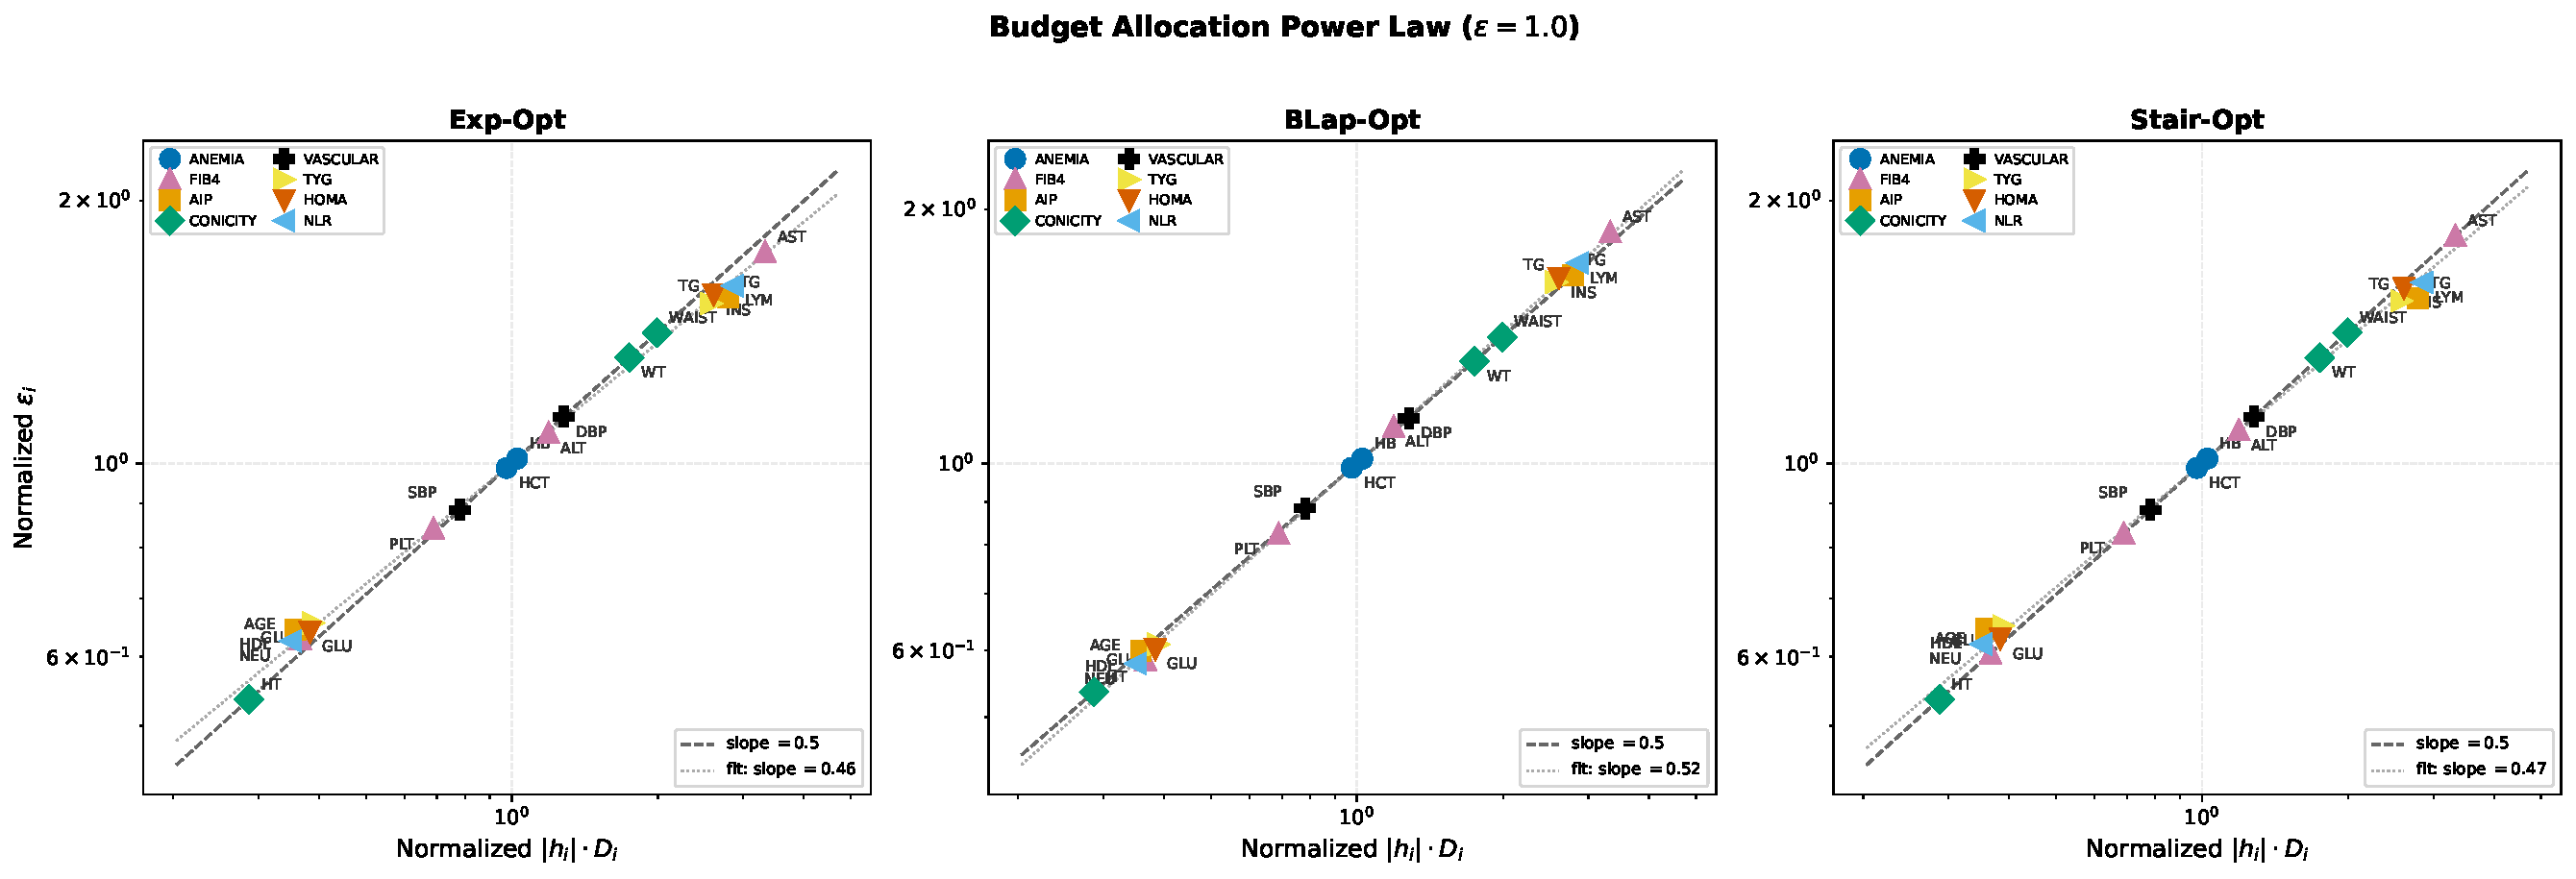
\includegraphics[width=\textwidth]{figures/rq2_allocation_powerlaw_eps1p0.pdf}
\caption{Log-log scatter of normalized per-root budget $\varepsilon_i$ vs.\ sensitivity--domain product $|h_i| \cdot D_i$ at $\varepsilon = 0.1$.  Each panel uses one mechanism's optimizer.  All three produce the same power law $\varepsilon_i \propto (|h_i| \cdot D_i)^{0.5}$ (dashed line; fitted slopes 0.46, 0.52, 0.47).  Hollow markers indicate floor-clamped roots with zero target sensitivity.}
\label{fig:allocation_powerlaw_10}
\end{figure*}

\begin{figure*}[t]
\centering
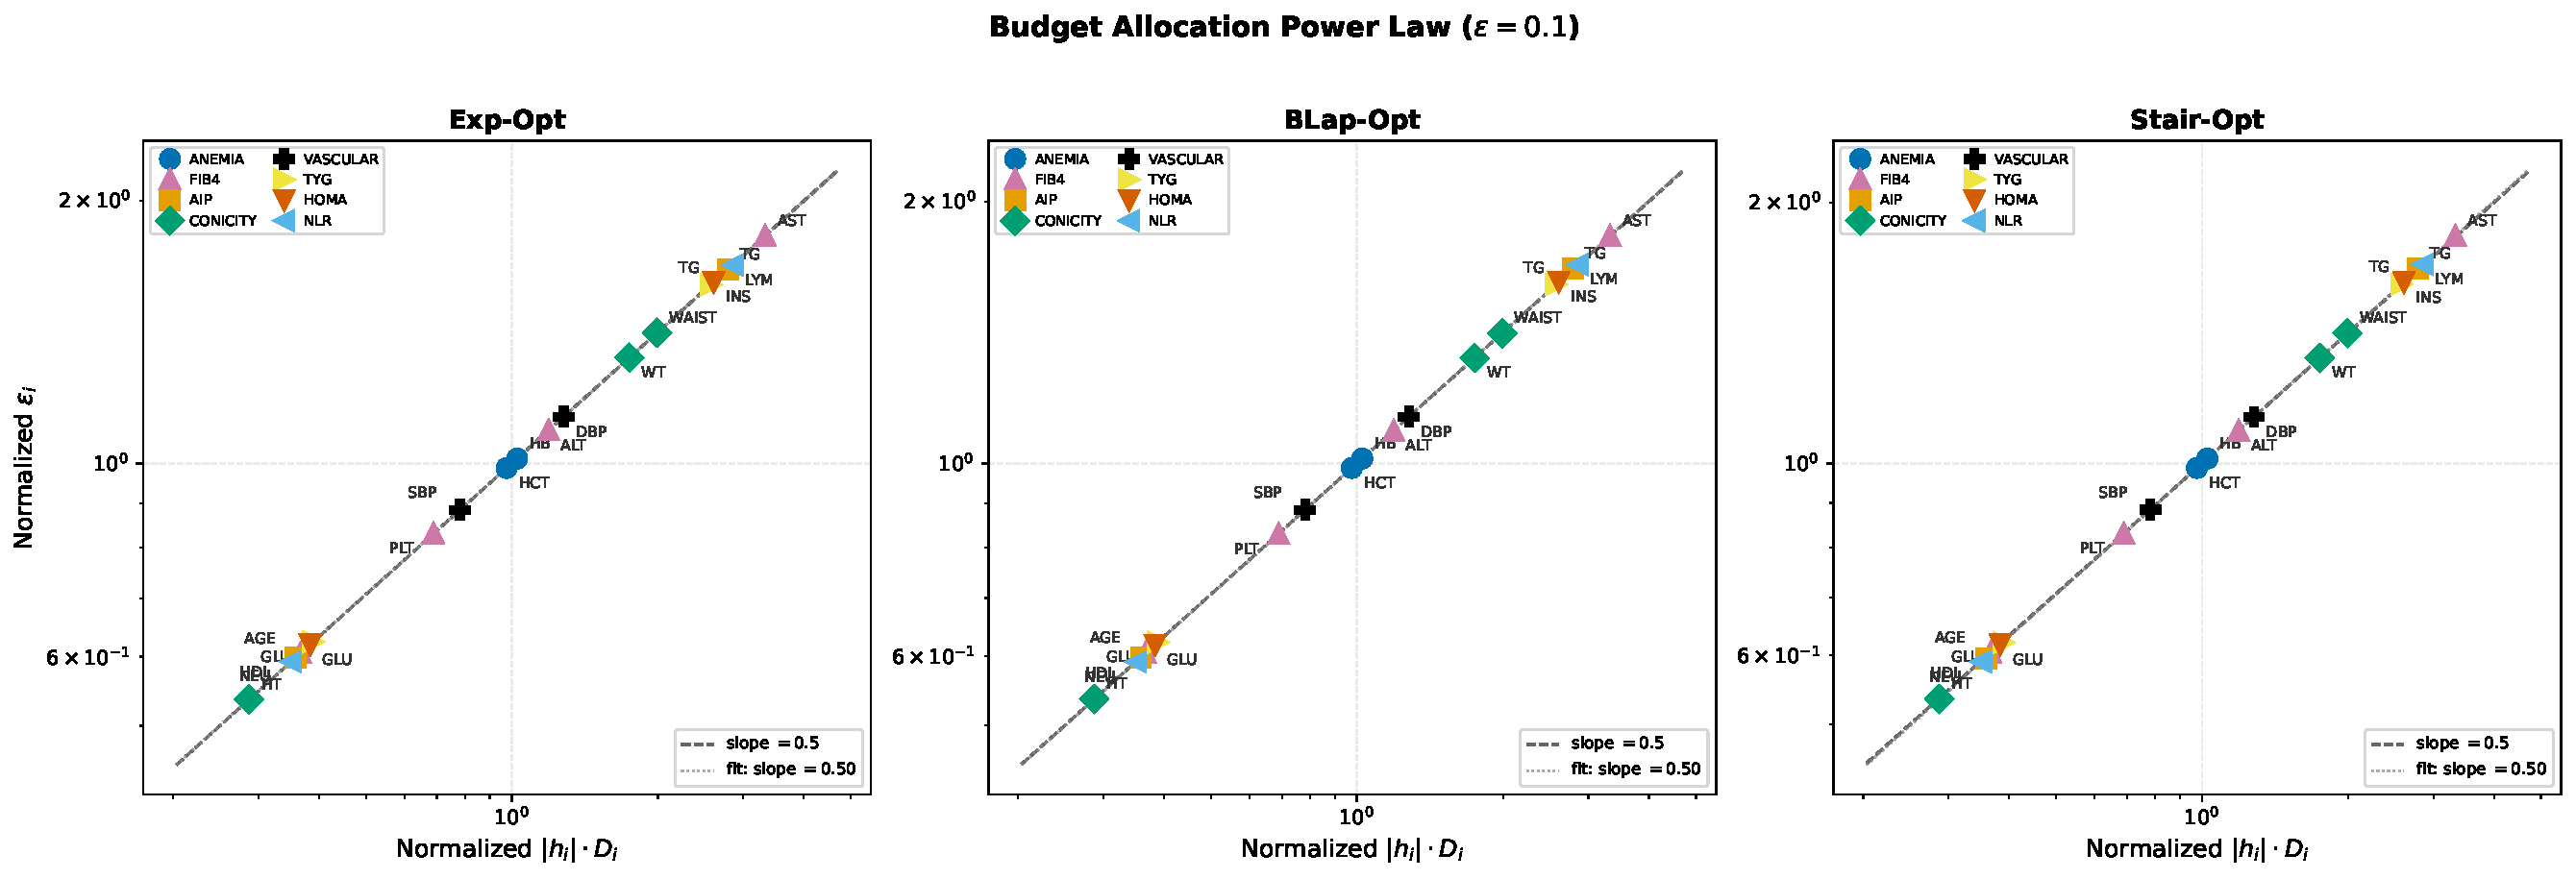
\includegraphics[width=\textwidth]{figures/rq2_allocation_powerlaw_eps0p1.pdf}
\caption{Log-log scatter of normalized per-root budget $\varepsilon_i$ vs.\ sensitivity--domain product $|h_i| \cdot D_i$ at $\varepsilon = 0.1$.  Each panel uses one mechanism's optimizer.  All three produce the same power law $\varepsilon_i \propto (|h_i| \cdot D_i)^{0.5}$ (dashed line; fitted slopes 0.50, 0.50, 0.50).  Hollow markers indicate floor-clamped roots with zero target sensitivity.}
\label{fig:allocation_powerlaw_01}
\end{figure*}

\subsection{Medical Profile Details}
\label{app:med-profiles}
\subsubsection*{1. Anemia Classification (MCHC)}
Red blood cell indices are derived from hemoglobin (Hb), hematocrit (Hct), and red blood cell count (RBC):
\begin{align}
\text{MCV} &= \frac{\text{Hct}}{\text{RBC}} \times 10, \quad
\text{MCH} = \frac{\text{Hb}}{\text{RBC}} \times 10, \quad
\text{MCHC} = \frac{\text{Hb}}{\text{Hct}} \times 100
\end{align}
These are the standard red cell indices defined in clinical hematology~\cite{hoffbrand2019essential}. The target value MCHC (mean corpuscular hemoglobin concentration, in g/dL) classifies chromicity: hypochromic ($\text{MCHC} < 32$), normochromic ($32 \leq \text{MCHC} \leq 36$), or hyperchromic ($\text{MCHC} > 36$)~\cite{buttarello2008automated}.

\subsubsection*{2. Liver Fibrosis (FIB-4)}
The FIB-4 index~\cite{sterling2006development} is a validated non-invasive biomarker for hepatic fibrosis staging:
\begin{equation}
\text{FIB-4} = \frac{\text{age} \times \text{AST}}{\text{PLT} \times \sqrt{\text{ALT}}}
\end{equation}
where AST and ALT are in U/L and PLT is in $10^9$/L. Risk thresholds: low risk/rule out ($\text{FIB-4} < 1.30$), indeterminate ($1.30 \leq \text{FIB-4} \leq 2.67$), high risk/rule in ($\text{FIB-4} > 2.67$). These cutoffs are from Sterling et al.~\cite{sterling2006development} and validated in subsequent NAFLD studies~\cite{mcpherson2017age}.

\subsubsection*{3. Atherogenic Index of Plasma (AIP)}
Lipid-derived values include non-HDL cholesterol ($\text{TC} - \text{HDL}$) and Friedewald LDL ($\text{TC} - \text{HDL} - \text{TG}/5$)~\cite{friedewald1972estimation}. The atherogenic index of plasma~\cite{dobiasova2001atherogenic} is:
\begin{equation}
\text{AIP} = \log_{10}\!\left(\frac{\text{TG}}{\text{HDL}}\right)
\end{equation}
where TG and HDL are in mg/dL. Risk classification: low cardiovascular risk ($\text{AIP} < 0.11$), intermediate ($0.11 \leq \text{AIP} \leq 0.21$), high ($\text{AIP} > 0.21$)~\cite{dobiasova2004atherogenic}.

\subsubsection*{4. Conicity Index (Obesity)}
Body composition is assessed via BMI ($\text{wt}/\text{ht}^2$), waist-to-height ratio ($\text{waist}/\text{ht}$), and the conicity index~\cite{valdez1991simple}:
\begin{equation}
\text{CI} = \frac{\text{waist}}{0.109 \times \sqrt{\text{wt}/\text{ht}}}
\end{equation}
where waist and height are in meters, and weight is in kilograms. The denominator represents the circumference of a cylinder with the same height and mass. Central obesity is indicated when $\text{CI} > 1.25$~\cite{pitanga2005sensitivity}.

\subsubsection*{5. Vascular Stiffness (Pulse Pressure Index)}
Blood pressure derivatives include pulse pressure ($\text{PP} = \text{SBP} - \text{DBP}$), mean arterial pressure ($\text{MAP} = \text{DBP} + \text{PP}/3$), and mid-blood pressure ($\text{MBP} = (\text{SBP} + \text{DBP})/2$). The pulse pressure index~\cite{kovaite2008arterial}:
\begin{equation}
\text{PPI} = \frac{\text{PP}}{\text{SBP}} = \frac{\text{SBP} - \text{DBP}}{\text{SBP}}
\end{equation}
High arterial stiffness is indicated when $\text{PPI} > 0.60$~\cite{franklin2009predictive}.

\subsubsection*{6. Triglyceride-Glucose Index (TyG)}
The TyG index~\cite{simental2008triglyceride} is a surrogate marker for insulin resistance:
\begin{equation}
\text{TyG} = \ln\!\left(\frac{\text{TG} \times \text{Glu}}{2}\right)
\end{equation}
where TG is in mg/dL and Glu is fasting glucose in mg/dL. Insulin resistance is indicated when $\text{TyG} > 8.5$~\cite{guerrero2010product}.

\subsubsection*{7. HOMA-IR (Insulin Resistance)}
The Homeostatic Model Assessment for Insulin Resistance~\cite{matthews1985homeostasis}:
\begin{equation}
\text{HOMA-IR} = \frac{\text{Glu} \times \text{Ins}}{405}
\end{equation}
where Glu is fasting glucose (mg/dL) and Ins is fasting insulin ($\mu$U/mL). The constant 405 normalizes to conventional units. Classification: insulin sensitive ($\text{HOMA} < 1.0$), normal ($1.0 \leq \text{HOMA} < 2.5$), insulin resistant ($\text{HOMA} \geq 2.5$)~\cite{gayoso2016homa}.

\subsubsection*{8. Neutrophil-to-Lymphocyte Ratio (NLR)}
The NLR is a marker of systemic inflammation~\cite{zahorec2001ratio}:
\begin{equation}
\text{NLR} = \frac{\text{Neutrophils}}{\text{Lymphocytes}}
\end{equation}
with auxiliary values $\text{NLR}_{\text{sum}} = \text{Neu} + \text{Lym}$ and $\text{NLR}_{\text{diff}} = |\text{Neu} - \text{Lym}|$ included as intermediate nodes. Systemic inflammation or physiologic stress is indicated when $\text{NLR} \geq 3.0$~\cite{forget2017normal}.


\subsection{Additional Baseline Details}
\label{app:baselines}
\subsubsection{\textbf{Discrete Exponential Mechanism}}
\label{app:exp-noise}

The mechanism samples index $s \in \{0, \dots, m{-}1\}$ with probability
\[
    P_{t_i}(s) = \frac{\alpha_i^{|t_i - s|}}{\sum_{r=0}^{m-1} \alpha_i^{|t_i - r|}}, \qquad \alpha_i = \exp(-\epsilon_i/2).
\]
The expected absolute noise in index units at position $t_i$ is:
\begin{equation}
\label{eq:bar-eta-discrete}
    \mathbb{E}[|s - t_i|] = \frac{\sum_{s=0}^{m-1} |t_i - s|\,\alpha_i^{|t_i - s|}}{\sum_{s=0}^{m-1} \alpha_i^{|t_i - s|}}.
\end{equation}
In domain units: $\bar{\eta}_i^{\,\mathrm{Exp}}(\epsilon_i) = \delta_i \cdot \mathbb{E}[|s - t_i|]$. Evaluated at the grid center $t_i = (m{-}1)/2$, where both tails have full support.
%% -----------------------------------------------------------------

\subsubsection{\textbf{Bounded Laplace}}
\label{app:blap-alloc}
The Bounded Laplace mechanism sanitizes root $i$ as follows. The true value $x_i$ is mapped to index space via $t_i = (x_i - \ell_i)/\delta_i$. Continuous noise is drawn from a Laplace distribution:
\[
    \tilde{t}_i = t_i + Z, \qquad Z \sim \mathrm{Lap}(0, 1/\epsilon_i),
\]
with density $p(z) = (\epsilon_i / 2)\exp(-\epsilon_i |z|)$. The noisy index is clamped and rounded:
\[
    s = \mathrm{round} \big(\mathrm{clip}(\tilde{t}_i,\; 0,\; m{-}1)\big).
\]
The output is $x'_i = s\,\delta_i + \ell_i$.
%% -----------------------------------------------------------------

\subsubsection{\textbf{Staircase Mechanism}}
\label{app:stair-alloc}

The Staircase mechanism~\cite{geng2015optimal} replaces the Laplace's smooth exponential density with a piecewise-constant density. For sensitivity $\Delta = 1$ in index space and privacy parameter $\epsilon_i$, the noise $\hat{\eta}_i$ is sampled as follows:
\begin{enumerate}
    \item Draw a sign $S \in \{-1, +1\}$ uniformly at random.
    \item Draw $G \sim \mathrm{Geom}(1 - e^{-\epsilon_i})$, with $\Pr[G = g] = (1 - e^{-\epsilon_i})\,e^{-\epsilon_i g}$ for $g = 0, 1, 2, \ldots$\; The integer $G$ selects which ``step'' the noise lands on: the noise magnitude will fall in the interval $[G,\, G{+}1)$ in index units.
    \item Draw $U \sim \mathrm{Uniform}(0, 1)$.
    \item With probability $\gamma = 1/(1 + e^{\epsilon_i/2})$: set $\hat{\eta}_i = S \cdot (G + U)$.\\
          With probability $1 - \gamma$: set $\hat{\eta}_i = S \cdot (G + 1 - U)$.
\end{enumerate}

\noindent The geometric variable $G$ determines the step, with each successive step having probability $e^{-\epsilon_i}$ times the previous --- the same decay rate as the Laplace. The uniform variable $U$ places the noise within the step. The $\gamma$-branch orients $U$ toward the inner edge (closer to zero); the $(1{-}\gamma)$-branch orients it toward the outer edge. The parameter $\gamma = 1/(1 + e^{\epsilon_i/2})$ balances these orientations.

The continuous noise is clamped to $[0, m{-}1]$ and rounded to the nearest grid point. The output in domain units is $\eta_i = (s - t_i)\,\delta_i$.

\subsection{Per-template win rates}
\label{app:rq3-winrate}
 
Table~\ref{tab:rq1_win_rate} reports the per-template win rate of $\mathcal{M}$-Opt over $\mathcal{M}$-All across all mechanisms and privacy levels. Under the unified single-draw root-based protocol (Sec.~\ref{sec:experiments-rq1}), $\mathcal{M}$-Opt wins on essentially every (template, mechanism, $\varepsilon$) cell at every budget level: $98\%$ at $B = (k{+}1)\varepsilon$ and $> 99\%$ at the larger budgets. The remaining few losses concentrate on NLR at very low $\varepsilon$, where wMAPE is already saturated above $80\%$ and bootstrap intervals overlap.
 
\begin{table}[t]
\centering
\small
\caption{$\mathcal{M}$-Opt vs.\ $\mathcal{M}$-All win rate per template (across 3 mechanisms $\times$ 10 $\varepsilon$ values = 30 pairs). A ``win'' means $\mathcal{M}$-Opt achieves lower wMAPE.}
\label{tab:rq1_win_rate}
\begin{tabular}{lcccc}
\toprule
\textbf{Template} & $k$ & $k{+}1$ & $2k{+}1$ & $3k{+}1$ \\
\midrule
ANEMIA   & 3 & 30/30 & 30/30 & 30/30 \\
FIB4     & 4 & 30/30 & 30/30 & 30/30 \\
AIP      & 3 & 30/30 & 30/30 & 30/30 \\
CONICITY & 3 & 30/30 & 30/30 & 30/30 \\
VASCULAR & 2 & 30/30 & 30/30 & 30/30 \\
TYG      & 2 & 30/30 & 30/30 & 30/30 \\
HOMA     & 2 & 30/30 & 30/30 & 30/30 \\
NLR      & 2 & 26/30 & 29/30 & 29/30 \\
\midrule
\textbf{Total} & & 236/240 (98\%) & 239/240 (>99\%) & 239/240 (>99\%) \\
\bottomrule
\end{tabular}
\end{table}

% ============================================================
% APPENDIX: Win rate table (moved from main text)
% ============================================================
% \subsection{Per-template win rates}
% \label{app:rq3-winrate}
 
% Table~\ref{tab:rq1_win_rate} reports the per-template win rate of $\mathcal{M}$-Opt over $\mathcal{M}$-All across all mechanisms and privacy levels. Templates are grouped by the same compression/amplification structure discussed in Sec.~\ref{sec:per-template}: FIB4 and HOMA (compressing formulas) show near-universal wins, while ANEMIA, TYG, and NLR (amplifying formulas or narrow target domains) show mixed results at tight budgets. The win rate grows monotonically with the total budget $B$, consistent with the allocation converging to the closed-form optimum as $\varepsilon_{\min}$ becomes non-binding.
 
% \begin{table}[t]
% \centering
% \small
% \caption{$\mathcal{M}$-Opt vs.\ $\mathcal{M}$-All win rate per template (across 3 mechanisms $\times$ 10 $\varepsilon$ values = 30 pairs). A ``win'' means $\mathcal{M}$-Opt achieves lower wMAPE.}
% \label{tab:rq1_win_rate}
% \begin{tabular}{lcccc}
% \toprule
% \textbf{Template} & $k$ & $k{+}1$ & $2k{+}1$ & $3k{+}1$ \\
% \midrule
% FIB4     & 4 & 27/30 & 30/30 & 30/30 \\
% HOMA     & 2 & 30/30 & 30/30 & 30/30 \\
% VASCULAR & 2 &  3/30 & 27/30 & 28/30 \\
% AIP      & 3 &  2/30 &  9/30 & 21/30 \\
% NLR      & 2 &  2/30 &  3/30 &  9/30 \\
% TYG      & 2 &  0/30 &  1/30 &  5/30 \\
% CONICITY & 3 &  0/30 &  1/30 & 23/30 \\
% ANEMIA   & 3 &  0/30 &  0/30 & 10/30 \\
% \midrule
% \textbf{Total} & & 64/240 (27\%) & 101/240 (42\%) & 156/240 (65\%) \\
% \bottomrule
% \end{tabular}
% \end{table}


% \begin{table*}[t]
% \centering
% \setlength{\tabcolsep}{3pt}
% \footnotesize
% \caption{Reconstruction analysis at matched utility (Bounded Laplace mechanism, utility measured by wMAPE). For each template, we select $\varepsilon_{\mathcal{M}-\text{All}}$ values spanning high to low noise, then find $\varepsilon_{\mathcal{M}-\text{Opt}}$ yielding the closest utility for $\mathcal{M}$-Opt. $\Delta$ columns show the adversary's improvement over the naive error from the released sanitized values. Positive values indicate that the adversary gains from the MAP attack, so a lower $\Delta$ is better. The MAP columns (M) show the reconstruction MAE achieved by the MAP adversary (higher means that the mechanism is more robust). Values are calculated as means across roots for 200 samples.}
% \label{tab:recon_matched_blap}
% \resizebox{\textwidth}{!}{
% \begin{tabular}{rc|c|cc|cc|cc||rc|c|cc|cc|cc@{\hspace{4pt}\vrule\hspace{4pt}}rc|c|cc|cc|cc||rc|c|cc|cc|cc}
% \toprule
% \multicolumn{9}{c||}{$\mathcal{M}$-\textbf{All}} & \multicolumn{9}{c@{\hspace{4pt}\vrule\hspace{4pt}}}{$\mathcal{M}$-\textbf{Opt}} &
% \multicolumn{9}{c||}{$\mathcal{M}$-\textbf{All}} & \multicolumn{9}{c}{$\mathcal{M}$-\textbf{Opt}} \\
% $\varepsilon$ & Ut & Nv & $\Delta_\text{U}{\downarrow}$ & M$_\text{U}{\uparrow}$ & $\Delta_\text{I}{\downarrow}$ & M$_\text{I}{\uparrow}$ & $\Delta_\text{J}{\downarrow}$ & M$_\text{J}{\uparrow}$ &
% $\varepsilon$ & Ut & Nv & $\Delta_\text{U}{\downarrow}$ & M$_\text{U}{\uparrow}$ & $\Delta_\text{I}{\downarrow}$ & M$_\text{I}{\uparrow}$ & $\Delta_\text{J}{\downarrow}$ & M$_\text{J}{\uparrow}$ &
% $\varepsilon$ & Ut & Nv & $\Delta_\text{U}{\downarrow}$ & M$_\text{U}{\uparrow}$ & $\Delta_\text{I}{\downarrow}$ & M$_\text{I}{\uparrow}$ & $\Delta_\text{J}{\downarrow}$ & M$_\text{J}{\uparrow}$ &
% $\varepsilon$ & Ut & Nv & $\Delta_\text{U}{\downarrow}$ & M$_\text{U}{\uparrow}$ & $\Delta_\text{I}{\downarrow}$ & M$_\text{I}{\uparrow}$ & $\Delta_\text{J}{\downarrow}$ & M$_\text{J}{\uparrow}$ \\
% \midrule
% \multicolumn{18}{c@{\hspace{4pt}\vrule\hspace{4pt}}}{\textbf{ANEMIA}} & \multicolumn{18}{c}{\textbf{FIB4}} \\
% \midrule
% 0.005 & 4.4 & 16.4 & $+0.7$ & 15.7 & $+9.1$ & 7.3 & $+9.9$ & 6.5 & 0.01 & 4.0 & 15.5 & $+0.0$ & 15.5 & $+11.0$ & 4.6 & $+12.1$ & 3.4 &
% 0.1 & 28.3 & 5.7 & $+0.6$ & 5.1 & $+0.6$ & 5.1 & $+0.5$ & 5.2 & 0.02 & 28.8 & 12.0 & $+0.0$ & 12.0 & $-1.9$ & 13.9 & $-1.3$ & 13.3 \\
% 0.05 & 0.5 & 1.8 & $+0.6$ & 1.2 & $+0.7$ & 1.2 & $+0.7$ & 1.2 & 0.1 & 0.4 & 14.7 & $+0.0$ & 14.7 & $+11.7$ & 3.0 & $+12.8$ & 1.9 &
% 0.2 & 12.6 & 2.7 & $+0.3$ & 2.4 & $+0.3$ & 2.4 & $+0.3$ & 2.4 & 0.05 & 14.1 & 5.3 & $+0.0$ & 5.3 & $-0.2$ & 5.5 & $-0.6$ & 5.9 \\
% 0.2 & 0.1 & 0.5 & $+0.1$ & 0.3 & $+0.1$ & 0.3 & $+0.1$ & 0.3 & 0.5 & 0.1 & 14.1 & $+0.0$ & 14.1 & $+11.3$ & 2.9 & $+12.4$ & 1.7 &
% 0.5 & 5.5 & 1.1 & $+0.2$ & 0.9 & $+0.2$ & 0.9 & $+0.2$ & 0.9 & 0.1 & 5.0 & 2.6 & $+0.0$ & 2.6 & $-0.0$ & 2.6 & $-0.0$ & 2.6 \\
% 0.5 & 0.1 & 0.2 & $+0.1$ & 0.1 & $+0.1$ & 0.1 & $+0.1$ & 0.1 & 1.0 & 0.0 & 14.3 & $+0.0$ & 14.3 & $+11.5$ & 2.8 & $+12.6$ & 1.7 &
% 1.0 & 3.1 & 0.6 & $+0.1$ & 0.5 & $+0.1$ & 0.5 & $+0.1$ & 0.5 & 0.2 & 3.5 & 1.3 & $+0.0$ & 1.3 & $-0.0$ & 1.3 & $-0.0$ & 1.3 \\
% \midrule
% \multicolumn{18}{c@{\hspace{4pt}\vrule\hspace{4pt}}}{\textbf{AIP}} & \multicolumn{18}{c}{\textbf{CONICITY}} \\
% \midrule
% 0.005 & 113 & 98.3 & $+19.0$ & 79.4 & $+68.7$ & 29.6 & $+69.6$ & 28.7 & 0.005 & 93.4 & 54.4 & $+0.0$ & 54.4 & $+21.8$ & 32.7 & $+22.5$ & 31.9 &
% 0.02 & 2.2 & 5.2 & $+1.8$ & 3.5 & $+2.1$ & 3.2 & $+2.3$ & 2.9 & 0.02 & 2.6 & 2.3 & $+0.0$ & 2.3 & $-0.0$ & 2.3 & $+0.0$ & 2.3 \\
% 0.01 & 67.2 & 55.8 & $+22.0$ & 33.7 & $+30.7$ & 25.1 & $+31.7$ & 24.1 & 0.01 & 65.8 & 39.7 & $+0.0$ & 39.7 & $+13.4$ & 26.2 & $+14.3$ & 25.3 &
% 0.1 & 0.5 & 1.1 & $+0.4$ & 0.7 & $+0.4$ & 0.7 & $+0.4$ & 0.7 & 0.1 & 0.6 & 0.4 & $+0.0$ & 0.4 & $-0.0$ & 0.4 & $-0.0$ & 0.4 \\
% 0.1 & 6.4 & 8.2 & $+4.8$ & 3.4 & $+4.7$ & 3.4 & $+4.7$ & 3.5 & 0.1 & 7.6 & 23.8 & $+0.0$ & 23.8 & $+15.9$ & 8.0 & $+16.7$ & 7.1 &
% 0.2 & 0.2 & 0.5 & $+0.1$ & 0.3 & $+0.1$ & 0.3 & $+0.1$ & 0.3 & 0.2 & 0.3 & 0.2 & $+0.0$ & 0.2 & $-0.0$ & 0.2 & $-0.0$ & 0.2 \\
% 0.5 & 1.1 & 1.7 & $+1.1$ & 0.6 & $+1.1$ & 0.6 & $+1.1$ & 0.6 & 1.0 & 1.3 & 21.6 & $+0.0$ & 21.6 & $+15.2$ & 6.4 & $+16.0$ & 5.6 &
% 1.0 & 0.0 & 0.1 & $+0.0$ & 0.1 & $+0.0$ & 0.1 & $+0.0$ & 0.1 & 1.0 & 0.1 & 0.1 & $+0.0$ & 0.1 & $+0.0$ & 0.0 & $+0.0$ & 0.0 \\
% \midrule
% \multicolumn{18}{c@{\hspace{4pt}\vrule\hspace{4pt}}}{\textbf{VASCULAR}} & \multicolumn{18}{c}{\textbf{TYG}} \\
% \midrule
% 0.02 & 9.7 & 7.4 & $+2.4$ & 5.0 & $+3.1$ & 4.3 & $+3.0$ & 4.4 & 0.01 & 10.3 & 4.7 & $+0.0$ & 4.7 & $+0.0$ & 4.7 & $+0.0$ & 4.7 &
% 0.005 & 11.5 & 139 & $+48.8$ & 89.8 & $+101$ & 38.0 & $+101$ & 37.3 & 0.005 & 9.8 & 56.1 & $+0.0$ & 56.1 & $+11.5$ & 44.6 & $+13.2$ & 43.0 \\
% 0.1 & 1.9 & 1.6 & $+0.6$ & 0.9 & $+0.6$ & 0.9 & $+0.7$ & 0.9 & 0.05 & 2.0 & 0.9 & $+0.0$ & 0.9 & $+0.0$ & 0.9 & $+0.0$ & 0.9 &
% 0.01 & 6.1 & 71.3 & $+32.7$ & 38.6 & $+39.4$ & 31.9 & $+40.0$ & 31.3 & 0.01 & 7.5 & 32.2 & $+0.0$ & 32.2 & $-2.5$ & 34.7 & $-2.3$ & 34.6 \\
% 0.2 & 1.0 & 0.8 & $+0.3$ & 0.4 & $+0.3$ & 0.4 & $+0.3$ & 0.4 & 0.1 & 1.0 & 0.5 & $+0.0$ & 0.5 & $+0.0$ & 0.5 & $+0.0$ & 0.5 &
% 0.1 & 0.6 & 10.0 & $+5.6$ & 4.4 & $+5.6$ & 4.3 & $+5.6$ & 4.3 & 0.2 & 0.6 & 2.0 & $+0.0$ & 2.0 & $-0.0$ & 2.0 & $-0.0$ & 2.0 \\
% 1.0 & 0.2 & 0.2 & $+0.1$ & 0.1 & $+0.1$ & 0.1 & $+0.1$ & 0.1 & 0.5 & 0.3 & 0.1 & $+0.0$ & 0.1 & $+0.0$ & 0.1 & $+0.0$ & 0.1 &
% 0.5 & 0.1 & 2.1 & $+1.2$ & 0.9 & $+1.2$ & 0.9 & $+1.2$ & 0.9 & 1.0 & 0.1 & 0.5 & $+0.0$ & 0.5 & $+0.0$ & 0.5 & $+0.0$ & 0.5 \\
% \midrule
% \multicolumn{18}{c@{\hspace{4pt}\vrule\hspace{4pt}}}{\textbf{HOMA}} & \multicolumn{18}{c}{\textbf{NLR}} \\
% \midrule
% 0.02 & 90.6 & 41.6 & $+1.7$ & 39.9 & $+1.3$ & 40.2 & $+2.2$ & 39.3 & 0.005 & 100 & 57.2 & $+0.0$ & 57.2 & $+11.0$ & 46.3 & $+11.8$ & 45.4 &
% 0.005 & 127 & 214 & $+79.2$ & 134 & $+178$ & 35.9 & $+177$ & 36.1 & 0.005 & 153 & 90.1 & $+0.0$ & 90.1 & $+53.5$ & 36.6 & $+53.9$ & 36.2 \\
% 0.05 & 45.0 & 21.2 & $+2.4$ & 18.8 & $+0.1$ & 21.1 & $-0.5$ & 21.7 & 0.01 & 47.2 & 32.9 & $+0.0$ & 32.9 & $-6.7$ & 39.6 & $-6.6$ & 39.5 &
% 0.01 & 66.1 & 117 & $+37.9$ & 78.8 & $+83.1$ & 33.5 & $+82.5$ & 34.2 & 0.02 & 57.9 & 27.4 & $+0.0$ & 27.4 & $-0.0$ & 27.4 & $+0.0$ & 27.4 \\
% 0.2 & 13.9 & 5.7 & $+0.7$ & 5.0 & $+0.5$ & 5.1 & $+0.2$ & 5.4 & 0.05 & 13.3 & 8.1 & $+0.0$ & 8.1 & $-2.1$ & 10.2 & $-2.2$ & 10.3 &
% 0.1 & 8.5 & 15.3 & $+8.3$ & 7.0 & $+8.6$ & 6.7 & $+8.5$ & 6.8 & 0.1 & 11.4 & 5.4 & $+0.0$ & 5.4 & $-0.0$ & 5.4 & $-0.0$ & 5.4 \\
% 1.0 & 2.3 & 1.1 & $+0.2$ & 0.9 & $+0.2$ & 0.9 & $+0.2$ & 0.9 & 0.2 & 2.5 & 1.8 & $+0.0$ & 1.8 & $+0.0$ & 1.8 & $+0.0$ & 1.8 &
% 0.5 & 1.8 & 3.6 & $+2.1$ & 1.5 & $+2.1$ & 1.5 & $+2.1$ & 1.5 & 1.0 & 1.7 & 0.7 & $+0.0$ & 0.7 & $-0.0$ & 0.7 & $-0.0$ & 0.7 \\
% \bottomrule
% \end{tabular}
% }
% \end{table*}

% \begin{table*}[t]
% \centering
% \setlength{\tabcolsep}{3pt}
% \footnotesize
% \caption{Reconstruction analysis at matched utility (Staircase mechanism, utility measured by wMAPE). For each template, we select $\varepsilon_{\mathcal{M}-\text{All}}$ values spanning high to low noise, then find $\varepsilon_{\mathcal{M}-\text{Opt}}$ yielding the closest utility for $\mathcal{M}$-Opt. $\Delta$ columns show the adversary's improvement over the naive error from the released sanitized values. Positive values indicate that the adversary gains from the MAP attack, so a lower $\Delta$ is better. The MAP columns (M) show the reconstruction MAE achieved by the MAP adversary (higher means that the mechanism is more robust). Values are calculated as means across roots for 200 samples. 
% % Note: the staircase mechanism's PMF parameter $a = e^{\varepsilon}\gamma$ exceeds 1 when the per-node $\varepsilon > \ln\!\bigl(\frac{1+\sqrt{5}}{2}\bigr) \approx 0.96$, so we restrict $\varepsilon_{\mathcal{M}\text{-All}} \leq 0.5$ and $\varepsilon_{\mathcal{M}\text{-Opt}} \leq 0.2$.
% }
% \label{tab:recon_matched_stair}
% \resizebox{\textwidth}{!}{
% \begin{tabular}{rc|c|cc|cc|cc||rc|c|cc|cc|cc@{\hspace{4pt}\vrule\hspace{4pt}}rc|c|cc|cc|cc||rc|c|cc|cc|cc}
% \toprule
% \multicolumn{9}{c||}{$\mathcal{M}$-\textbf{All}} & \multicolumn{9}{c@{\hspace{4pt}\vrule\hspace{4pt}}}{$\mathcal{M}$-\textbf{Opt}} &
% \multicolumn{9}{c||}{$\mathcal{M}$-\textbf{All}} & \multicolumn{9}{c}{$\mathcal{M}$-\textbf{Opt}} \\
% $\varepsilon$ & Ut & Nv & $\Delta_\text{U}{\downarrow}$ & M$_\text{U}{\uparrow}$ & $\Delta_\text{I}{\downarrow}$ & M$_\text{I}{\uparrow}$ & $\Delta_\text{J}{\downarrow}$ & M$_\text{J}{\uparrow}$ &
% $\varepsilon$ & Ut & Nv & $\Delta_\text{U}{\downarrow}$ & M$_\text{U}{\uparrow}$ & $\Delta_\text{I}{\downarrow}$ & M$_\text{I}{\uparrow}$ & $\Delta_\text{J}{\downarrow}$ & M$_\text{J}{\uparrow}$ &
% $\varepsilon$ & Ut & Nv & $\Delta_\text{U}{\downarrow}$ & M$_\text{U}{\uparrow}$ & $\Delta_\text{I}{\downarrow}$ & M$_\text{I}{\uparrow}$ & $\Delta_\text{J}{\downarrow}$ & M$_\text{J}{\uparrow}$ &
% $\varepsilon$ & Ut & Nv & $\Delta_\text{U}{\downarrow}$ & M$_\text{U}{\uparrow}$ & $\Delta_\text{I}{\downarrow}$ & M$_\text{I}{\uparrow}$ & $\Delta_\text{J}{\downarrow}$ & M$_\text{J}{\uparrow}$ \\
% \midrule
% \multicolumn{18}{c@{\hspace{4pt}\vrule\hspace{4pt}}}{\textbf{ANEMIA}} & \multicolumn{18}{c}{\textbf{FIB4}} \\
% \midrule
% 0.005 & 4.4 & 17.4 & $+0.5$ & 17.0 & $+10.2$ & 7.2 & $+11.1$ & 6.3 & 0.01 & 4.5 & 16.2 & $+0.0$ & 16.2 & $+11.4$ & 4.8 & $+12.8$ & 3.5 &
% 0.005 & 263 & 74.1 & $+8.1$ & 66.0 & $+42.4$ & 31.8 & $+40.6$ & 33.5 & 0.005 & 258 & 41.3 & $+0.0$ & 41.3 & $+7.8$ & 33.5 & $+10.3$ & 31.0 \\
% 0.01 & 2.5 & 8.8 & $+2.5$ & 6.3 & $+3.4$ & 5.4 & $+4.3$ & 4.5 & 0.02 & 2.5 & 15.4 & $+0.0$ & 15.4 & $+11.5$ & 3.9 & $+12.6$ & 2.8 &
% 0.05 & 48.3 & 10.6 & $+1.1$ & 9.5 & $+1.0$ & 9.6 & $+1.3$ & 9.3 & 0.02 & 43.3 & 13.5 & $+0.0$ & 13.5 & $-1.8$ & 15.3 & $-1.2$ & 14.7 \\
% 0.05 & 0.5 & 1.7 & $+0.5$ & 1.3 & $+0.6$ & 1.1 & $+0.6$ & 1.1 & 0.1 & 0.4 & 14.4 & $+0.0$ & 14.4 & $+11.4$ & 3.0 & $+12.6$ & 1.9 &
% 0.2 & 13.9 & 2.4 & $+0.3$ & 2.1 & $+0.3$ & 2.1 & $+0.4$ & 2.0 & 0.05 & 12.5 & 4.9 & $+0.0$ & 4.9 & $-0.2$ & 5.1 & $-0.5$ & 5.4 \\
% 0.1 & 0.3 & 0.9 & $+0.3$ & 0.7 & $+0.3$ & 0.7 & $+0.3$ & 0.6 & 0.1 & 0.4 & 14.4 & $+0.0$ & 14.4 & $+11.4$ & 3.0 & $+12.6$ & 1.9 &
% 0.5 & 6.2 & 1.1 & $+0.1$ & 1.0 & $+0.1$ & 1.0 & $+0.1$ & 1.0 & 0.1 & 6.1 & 2.7 & $+0.0$ & 2.7 & $+0.0$ & 2.7 & $+0.0$ & 2.7 \\
% \midrule
% \multicolumn{18}{c@{\hspace{4pt}\vrule\hspace{4pt}}}{\textbf{AIP}} & \multicolumn{18}{c}{\textbf{CONICITY}} \\
% \midrule
% 0.005 & 126 & 115 & $+27.6$ & 87.8 & $+83.9$ & 31.6 & $+84.5$ & 30.9 & 0.005 & 98.4 & 54.1 & $+0.0$ & 54.1 & $+22.2$ & 31.9 & $+22.8$ & 31.3 &
% 0.005 & 8.1 & 17.6 & $+1.8$ & 15.8 & $+8.4$ & 9.2 & $+9.4$ & 8.2 & 0.01 & 6.8 & 4.9 & $+0.0$ & 4.9 & $+0.1$ & 4.8 & $+0.9$ & 4.0 \\
% 0.01 & 65.8 & 51.7 & $+20.0$ & 31.7 & $+28.5$ & 23.2 & $+29.9$ & 21.8 & 0.01 & 64.3 & 39.0 & $+0.0$ & 39.0 & $+12.8$ & 26.2 & $+13.8$ & 25.2 &
% 0.01 & 4.5 & 9.5 & $+2.2$ & 7.3 & $+3.5$ & 6.0 & $+3.9$ & 5.7 & 0.02 & 3.1 & 2.4 & $+0.0$ & 2.4 & $+0.0$ & 2.4 & $+0.0$ & 2.4 \\
% 0.1 & 6.9 & 7.4 & $+4.2$ & 3.2 & $+4.2$ & 3.2 & $+4.1$ & 3.3 & 0.1 & 7.8 & 24.5 & $+0.0$ & 24.5 & $+16.4$ & 8.2 & $+17.1$ & 7.4 &
% 0.05 & 0.9 & 2.0 & $+0.6$ & 1.4 & $+0.7$ & 1.3 & $+0.7$ & 1.4 & 0.05 & 1.2 & 0.9 & $+0.0$ & 0.9 & $-0.0$ & 0.9 & $+0.0$ & 0.9 \\
% 0.2 & 3.9 & 4.4 & $+2.7$ & 1.7 & $+2.7$ & 1.7 & $+2.7$ & 1.7 & 0.2 & 4.8 & 23.2 & $+0.0$ & 23.2 & $+15.8$ & 7.3 & $+16.7$ & 6.5 &
% 0.2 & 0.2 & 0.5 & $+0.2$ & 0.3 & $+0.2$ & 0.3 & $+0.2$ & 0.3 & 0.2 & 0.3 & 0.2 & $+0.0$ & 0.2 & $-0.0$ & 0.2 & $-0.0$ & 0.2 \\
% \midrule
% \multicolumn{18}{c@{\hspace{4pt}\vrule\hspace{4pt}}}{\textbf{VASCULAR}} & \multicolumn{18}{c}{\textbf{TYG}} \\
% \midrule
% 0.01 & 19.9 & 14.5 & $+4.4$ & 10.2 & $+7.0$ & 7.5 & $+7.1$ & 7.5 & 0.005 & 21.4 & 9.6 & $+0.0$ & 9.6 & $+0.9$ & 8.7 & $+1.1$ & 8.5 &
% 0.005 & 11.2 & 135 & $+52.7$ & 82.0 & $+98.6$ & 36.0 & $+99.0$ & 35.7 & 0.005 & 10.0 & 54.6 & $+0.0$ & 54.6 & $+12.0$ & 42.6 & $+12.9$ & 41.7 \\
% 0.02 & 10.4 & 7.2 & $+2.5$ & 4.7 & $+2.8$ & 4.4 & $+2.9$ & 4.2 & 0.01 & 9.7 & 4.6 & $+0.0$ & 4.6 & $+0.0$ & 4.5 & $+0.0$ & 4.6 &
% 0.01 & 6.5 & 77.9 & $+29.7$ & 48.2 & $+44.7$ & 33.2 & $+45.8$ & 32.1 & 0.01 & 6.8 & 33.4 & $+0.0$ & 33.4 & $-2.4$ & 35.8 & $-2.2$ & 35.6 \\
% 0.1 & 2.0 & 1.5 & $+0.6$ & 0.9 & $+0.6$ & 0.9 & $+0.6$ & 0.9 & 0.05 & 1.9 & 0.9 & $+0.0$ & 0.9 & $-0.0$ & 0.9 & $-0.0$ & 0.9 &
% 0.05 & 1.3 & 20.7 & $+12.0$ & 8.6 & $+12.0$ & 8.7 & $+11.9$ & 8.7 & 0.1 & 1.2 & 4.1 & $+0.0$ & 4.1 & $+0.0$ & 4.0 & $+0.0$ & 4.0 \\
% 0.2 & 0.9 & 0.7 & $+0.2$ & 0.4 & $+0.2$ & 0.4 & $+0.3$ & 0.4 & 0.1 & 1.1 & 0.5 & $+0.0$ & 0.5 & $+0.0$ & 0.5 & $+0.0$ & 0.5 &
% 0.1 & 0.7 & 11.5 & $+6.9$ & 4.7 & $+6.8$ & 4.8 & $+6.8$ & 4.8 & 0.2 & 0.6 & 2.0 & $+0.0$ & 2.0 & $-0.0$ & 2.1 & $-0.0$ & 2.1 \\
% \midrule
% \multicolumn{18}{c@{\hspace{4pt}\vrule\hspace{4pt}}}{\textbf{HOMA}} & \multicolumn{18}{c}{\textbf{NLR}} \\
% \midrule
% 0.02 & 112 & 42.4 & $+2.2$ & 40.2 & $+2.5$ & 39.9 & $+3.9$ & 38.5 & 0.005 & 88.4 & 52.3 & $+0.0$ & 52.3 & $+5.6$ & 46.7 & $+7.6$ & 44.7 &
% 0.005 & 122 & 216 & $+91.0$ & 125 & $+181$ & 34.8 & $+181$ & 34.6 & 0.01 & 108 & 48.6 & $+0.0$ & 48.6 & $+9.8$ & 38.8 & $+10.2$ & 38.4 \\
% 0.1 & 26.3 & 10.4 & $+1.2$ & 9.3 & $+0.0$ & 10.4 & $-0.2$ & 10.6 & 0.02 & 27.7 & 17.6 & $+0.0$ & 17.6 & $-5.7$ & 23.3 & $-6.1$ & 23.7 &
% 0.01 & 63.1 & 110 & $+28.8$ & 81.0 & $+79.4$ & 30.4 & $+78.9$ & 30.9 & 0.02 & 55.1 & 25.6 & $+0.0$ & 25.6 & $+0.5$ & 25.1 & $+0.5$ & 25.1 \\
% 0.2 & 14.3 & 4.9 & $+0.3$ & 4.6 & $-0.1$ & 5.0 & $-0.1$ & 5.0 & 0.05 & 12.1 & 7.8 & $+0.0$ & 7.8 & $-2.0$ & 9.8 & $-2.2$ & 10.0 &
% 0.05 & 18.0 & 29.3 & $+11.9$ & 17.4 & $+16.5$ & 12.8 & $+16.6$ & 12.7 & 0.05 & 25.3 & 11.2 & $+0.0$ & 11.2 & $+0.1$ & 11.1 & $+0.2$ & 11.1 \\
% 0.5 & 6.0 & 2.0 & $+0.3$ & 1.7 & $+0.3$ & 1.7 & $+0.2$ & 1.8 & 0.1 & 6.0 & 3.9 & $+0.0$ & 3.9 & $+0.1$ & 3.8 & $+0.0$ & 3.8 &
% 0.1 & 8.4 & 16.4 & $+8.5$ & 7.8 & $+9.2$ & 7.2 & $+9.1$ & 7.3 & 0.2 & 6.8 & 3.1 & $+0.0$ & 3.1 & $+0.0$ & 3.1 & $-0.0$ & 3.1 \\
% \bottomrule
% \end{tabular}
% }
% \end{table*}


% Appendix subsection: Reconstruction tables for RQ2
% Reference target: app:rq2-tables (used in Sec 5.3 of main text)

\subsection{Reconstruction Attack Results (RQ2)}
\label{app:rq2-tables}
\label{app:reconstruction}

This appendix supports the claims of Sec.~\ref{sec:experiments-rq2} with three pieces of evidence: (i) a per-template breakdown showing that $\mathcal{M}$-All's reconstruction wMAPE degrades with query count on every template under the focal condition (Exponential, Strategy B, informed prior, $\varepsilon_r = 0.1$); (ii) Exponential aggregates under Strategy A and Strategy B for both priors, across all five privacy levels; (iii) aggregate reconstruction wMAPE for the Bounded Laplace and Staircase mechanisms under Strategy B (informed prior), confirming the same pattern observed for the Exponential mechanism (Table~\ref{tab:recon_main} in the main text). Bootstrap details and the full appendix (per-mechanism, per-strategy, per-prior, per-template at every $\varepsilon_r$) are in the supplementary material.

\paragraph{Per-template results (Exponential, $\varepsilon_r = 0.1$, Strategy B, informed prior).}
Table~\ref{tab:rq2_per_template} reports per-template reconstruction wMAPE under Strategy B with the informed prior at $\varepsilon_r = 0.1$. $\mathcal{M}$-All degrades monotonically with $q$ on every template; $\mathcal{M}$-Roots and $\mathcal{M}$-Opt are invariant. The largest absolute degradations occur on templates with wide root domains (HOMA, NLR, TYG).

\begin{table}[h]
\centering
\setlength{\tabcolsep}{3pt}
\small
\caption{Per-template reconstruction wMAPE (\%) at $\varepsilon_r = 0.1$ (Exponential, Strategy B, informed prior). $\mathcal{M}$-All degrades monotonically with $q$ on every template; $\mathcal{M}$-Roots and $\mathcal{M}$-Opt are invariant to $q$ (single value shown).}
\label{tab:rq2_per_template}
\begin{tabular}{l|cccc|cc}
\toprule
& \multicolumn{4}{c|}{$\mathcal{M}$-All} & $\mathcal{M}$-Roots & $\mathcal{M}$-Opt \\
\textbf{Template} & $q{=}1$ & $q{=}4$ & $q{=}8$ & $q{=}16$ & (any $q$) & (any $q$) \\
\midrule
ANEMIA   & 1.6  & 0.8  & 0.6  & 0.4  & 1.9  & 3.6 \\
FIB4     & 8.5  & 4.9  & 3.4  & 2.4  & 10.2 & 9.3 \\
AIP      & 11.2 & 7.2  & 5.6  & 3.9  & 15.0 & 14.3 \\
CONICITY & 2.1  & 0.9  & 0.7  & 0.5  & 2.2  & 1.9 \\
VASCULAR & 2.5  & 1.3  & 0.9  & 0.6  & 2.7  & 2.7 \\
TYG      & 15.5 & 11.0 & 7.3  & 5.0  & 20.4 & 17.3 \\
HOMA     & 19.1 & 9.7  & 6.9  & 5.1  & 24.3 & 20.5 \\
NLR      & 20.9 & 17.2 & 10.5 & 7.6  & 28.8 & 25.6 \\
\bottomrule
\end{tabular}
\end{table}

\paragraph{Exponential: Strategy A and Strategy B aggregates (both priors).}
Tables~\ref{tab:rq2_exp_A_uniform}--\ref{tab:rq2_exp_B_informed} report aggregate reconstruction wMAPE for the Exponential mechanism across all five privacy levels under both strategies and both priors. Under Strategy A (single targeted root $r^*$), $\mathcal{M}$-All has $q+1$ observations on $r^*$ at each $q$ and the gap to $\mathcal{M}$-Roots widens monotonically; under Strategy B (queries distributed across all roots), the same pattern holds for the average across roots. The informed prior gives qualitatively identical behavior to uniform — under v3 there is no target-release coupling, so the prior contributes only soft regularization.

\begin{table}[h]
\centering
\setlength{\tabcolsep}{2.5pt}
\small
\caption{Exponential, Strategy A, uniform prior: aggregate reconstruction wMAPE (\%) (mean across 8 templates). Reports the targeted root $r^*$ only.}
\label{tab:rq2_exp_A_uniform}
\begin{tabular}{c|ccc|ccc|ccc|ccc}
\toprule
& \multicolumn{3}{c|}{$q=1$} & \multicolumn{3}{c|}{$q=4$} & \multicolumn{3}{c|}{$q=8$} & \multicolumn{3}{c}{$q=16$} \\
$\varepsilon_r$ & All & Rts & Opt & All & Rts & Opt & All & Rts & Opt & All & Rts & Opt \\
\midrule
0.01 & 127  & 213  & 104  & 97.2 & 213  & 104  & 74.7 & 213  & 104  & 55.4 & 213  & 104 \\
0.05 & 26.1 & 42.4 & 27.9 & 23.3 & 42.4 & 27.9 & 16.9 & 42.4 & 27.9 & 12.3 & 42.4 & 27.9 \\
0.1  & 16.5 & 22.4 & 15.1 & 12.3 & 22.4 & 15.1 & 8.6  & 22.4 & 15.1 & 5.9  & 22.4 & 15.1 \\
0.5  & 4.9  & 5.3  & 3.4  & 2.3  & 5.3  & 3.4  & 1.7  & 5.3  & 3.4  & 1.1  & 5.3  & 3.4 \\
1.0  & 2.5  & 2.7  & 1.7  & 1.2  & 2.7  & 1.7  & 0.9  & 2.7  & 1.7  & 0.6  & 2.7  & 1.7 \\
\bottomrule
\end{tabular}
\end{table}

\begin{table}[h]
\centering
\setlength{\tabcolsep}{2.5pt}
\small
\caption{Exponential, Strategy A, informed prior: aggregate reconstruction wMAPE (\%) (mean across 8 templates). Targeted root only.}
\label{tab:rq2_exp_A_informed}
\begin{tabular}{c|ccc|ccc|ccc|ccc}
\toprule
& \multicolumn{3}{c|}{$q=1$} & \multicolumn{3}{c|}{$q=4$} & \multicolumn{3}{c|}{$q=8$} & \multicolumn{3}{c}{$q=16$} \\
$\varepsilon_r$ & All & Rts & Opt & All & Rts & Opt & All & Rts & Opt & All & Rts & Opt \\
\midrule
0.01 & 35.4 & 38.4 & 44.8 & 34.7 & 38.4 & 44.8 & 34.1 & 38.4 & 44.8 & 32.5 & 38.4 & 44.8 \\
0.05 & 28.3 & 40.3 & 29.1 & 19.7 & 40.3 & 29.1 & 15.6 & 40.3 & 29.1 & 11.7 & 40.3 & 29.1 \\
0.1  & 17.8 & 23.8 & 15.9 & 12.3 & 23.8 & 15.9 & 8.3  & 23.8 & 15.9 & 5.9  & 23.8 & 15.9 \\
0.5  & 5.0  & 5.3  & 3.4  & 2.3  & 5.3  & 3.4  & 1.7  & 5.3  & 3.4  & 1.1  & 5.3  & 3.4 \\
1.0  & 2.6  & 2.7  & 1.7  & 1.2  & 2.7  & 1.7  & 0.9  & 2.7  & 1.7  & 0.6  & 2.7  & 1.7 \\
\bottomrule
\end{tabular}
\end{table}

\begin{table}[h]
\centering
\setlength{\tabcolsep}{2.5pt}
\small
\caption{Exponential, Strategy B, uniform prior: aggregate reconstruction wMAPE (\%) (mean across 8 templates). Reports the average across all $k$ roots.}
\label{tab:rq2_exp_B_uniform}
\begin{tabular}{c|ccc|ccc|ccc|ccc}
\toprule
& \multicolumn{3}{c|}{$q=1$} & \multicolumn{3}{c|}{$q=4$} & \multicolumn{3}{c|}{$q=8$} & \multicolumn{3}{c}{$q=16$} \\
$\varepsilon_r$ & All & Rts & Opt & All & Rts & Opt & All & Rts & Opt & All & Rts & Opt \\
\midrule
0.01 & 73.8 & 115  & 84.9 & 54.5 & 115  & 84.9 & 41.7 & 115  & 84.9 & 30.7 & 115  & 84.9 \\
0.05 & 16.6 & 23.8 & 22.4 & 12.6 & 23.8 & 22.4 & 9.2  & 23.8 & 22.4 & 6.6  & 23.8 & 22.4 \\
0.1  & 9.9  & 12.5 & 13.5 & 6.6  & 12.5 & 13.5 & 4.7  & 12.5 & 13.5 & 3.2  & 12.5 & 13.5 \\
0.5  & 2.7  & 2.9  & 5.5  & 1.3  & 2.9  & 5.5  & 0.9  & 2.9  & 5.5  & 0.6  & 2.9  & 5.5 \\
1.0  & 1.3  & 1.5  & 4.3  & 0.7  & 1.5  & 4.3  & 0.5  & 1.5  & 4.3  & 0.3  & 1.5  & 4.3 \\
\bottomrule
\end{tabular}
\end{table}

\begin{table}[h]
\centering
\setlength{\tabcolsep}{2.5pt}
\small
\caption{Exponential, Strategy B, informed prior: aggregate reconstruction wMAPE (\%) (mean across 8 templates). This is the focal condition reported in main-text Table~\ref{tab:recon_main}.}
\label{tab:rq2_exp_B_informed}
\begin{tabular}{c|ccc|ccc|ccc|ccc}
\toprule
& \multicolumn{3}{c|}{$q=1$} & \multicolumn{3}{c|}{$q=4$} & \multicolumn{3}{c|}{$q=8$} & \multicolumn{3}{c}{$q=16$} \\
$\varepsilon_r$ & All & Rts & Opt & All & Rts & Opt & All & Rts & Opt & All & Rts & Opt \\
\midrule
0.01 & 24.7 & 28.8 & 30.3 & 23.3 & 28.8 & 30.3 & 21.6 & 28.8 & 30.3 & 19.6 & 28.8 & 30.3 \\
0.05 & 16.4 & 22.8 & 21.0 & 10.9 & 22.8 & 21.0 & 8.6  & 22.8 & 21.0 & 6.4  & 22.8 & 21.0 \\
0.1  & 10.2 & 13.2 & 11.9 & 6.6  & 13.2 & 11.9 & 4.5  & 13.2 & 11.9 & 3.2  & 13.2 & 11.9 \\
0.5  & 2.8  & 2.9  & 3.4  & 1.3  & 2.9  & 3.4  & 0.9  & 2.9  & 3.4  & 0.6  & 2.9  & 3.4 \\
1.0  & 1.4  & 1.5  & 2.3  & 0.7  & 1.5  & 2.3  & 0.5  & 1.5  & 2.3  & 0.3  & 1.5  & 2.3 \\
\bottomrule
\end{tabular}
\end{table}

\paragraph{Bounded Laplace and Staircase aggregates (Strategy B, informed prior).}
Tables~\ref{tab:rq2_blap_agg} and~\ref{tab:rq2_stair_agg} report aggregate reconstruction wMAPE for the Bounded Laplace and Staircase mechanisms under the focal condition (Strategy B, informed prior, mean across 8 templates). Both follow the same pattern as Exponential: $\mathcal{M}$-All decreases with $q$ at every $\varepsilon_r$, while $\mathcal{M}$-Roots and $\mathcal{M}$-Opt are invariant.

\begin{table}[h]
\centering
\setlength{\tabcolsep}{2.5pt}
\small
\caption{Bounded Laplace, Strategy B, informed prior: aggregate reconstruction wMAPE (\%) (mean across 8 templates).}
\label{tab:rq2_blap_agg}
\begin{tabular}{c|ccc|ccc|ccc|ccc}
\toprule
& \multicolumn{3}{c|}{$q=1$} & \multicolumn{3}{c|}{$q=4$} & \multicolumn{3}{c|}{$q=8$} & \multicolumn{3}{c}{$q=16$} \\
$\varepsilon_r$ & All & Rts & Opt & All & Rts & Opt & All & Rts & Opt & All & Rts & Opt \\
\midrule
0.01 & 25.9 & 31.1 & 32.4 & 23.4 & 31.1 & 32.4 & 24.0 & 31.1 & 32.4 & 23.1 & 31.1 & 32.4 \\
0.05 & 11.5 & 13.5 & 12.2 & 7.7  & 13.5 & 12.2 & 6.3  & 13.5 & 12.2 & 5.4  & 13.5 & 12.2 \\
0.1  & 6.6  & 7.2  & 6.8  & 3.5  & 7.2  & 6.8  & 2.7  & 7.2  & 6.8  & 2.0  & 7.2  & 6.8 \\
0.5  & 1.4  & 1.5  & 2.3  & 0.7  & 1.5  & 2.3  & 0.5  & 1.5  & 2.3  & 0.4  & 1.5  & 2.3 \\
1.0  & 0.7  & 0.8  & 1.7  & 0.4  & 0.8  & 1.7  & 0.3  & 0.8  & 1.7  & 0.2  & 0.8  & 1.7 \\
\bottomrule
\end{tabular}
\end{table}

\begin{table}[h]
\centering
\setlength{\tabcolsep}{2.5pt}
\small
\caption{Staircase, Strategy B, informed prior: aggregate reconstruction wMAPE (\%) (mean across 8 templates). $\varepsilon_r = 1.0$ omitted (mechanism degenerate at high budget).}
\label{tab:rq2_stair_agg}
\begin{tabular}{c|ccc|ccc|ccc|ccc}
\toprule
& \multicolumn{3}{c|}{$q=1$} & \multicolumn{3}{c|}{$q=4$} & \multicolumn{3}{c|}{$q=8$} & \multicolumn{3}{c}{$q=16$} \\
$\varepsilon_r$ & All & Rts & Opt & All & Rts & Opt & All & Rts & Opt & All & Rts & Opt \\
\midrule
0.01 & 25.8 & 30.4 & 31.4 & 23.7 & 30.4 & 31.4 & 23.7 & 30.4 & 31.4 & 23.2 & 30.4 & 31.4 \\
0.05 & 11.6 & 13.6 & 12.0 & 7.8  & 13.6 & 12.0 & 6.6  & 13.6 & 12.0 & 5.6  & 13.6 & 12.0 \\
0.1  & 6.6  & 7.1  & 6.6  & 3.5  & 7.1  & 6.6  & 2.7  & 7.1  & 6.6  & 2.1  & 7.1  & 6.6 \\
0.5  & 1.5  & 1.4  & 1.6  & 0.7  & 1.4  & 1.6  & 0.5  & 1.4  & 1.6  & 0.4  & 1.4  & 1.6 \\
\bottomrule
\end{tabular}
\end{table}


\subsection{RQ1: Per-template wMAPE Curves}
\label{app:rq1-tables-figs}

Fig.~\ref{fig:per_template_app} shows the per-template wMAPE for all 8 medical
templates across the full $\varepsilon$ sweep at $B = (2k{+}1)\varepsilon$.
Templates are arranged in two rows by absolute-gap regime (Sec.~\ref{sec:experiments-rq3}):
the top row contains compressing-formula templates with the largest absolute
$\mathcal{M}$-All vs.\ \sysname{} gaps; the bottom row contains amplifying-formula
templates with smaller absolute gaps but comparable multiplicative ratios. Each
panel overlays nine methods (3 mechanisms $\times$ 3 configurations).

\begin{figure*}[t]
    \centering
    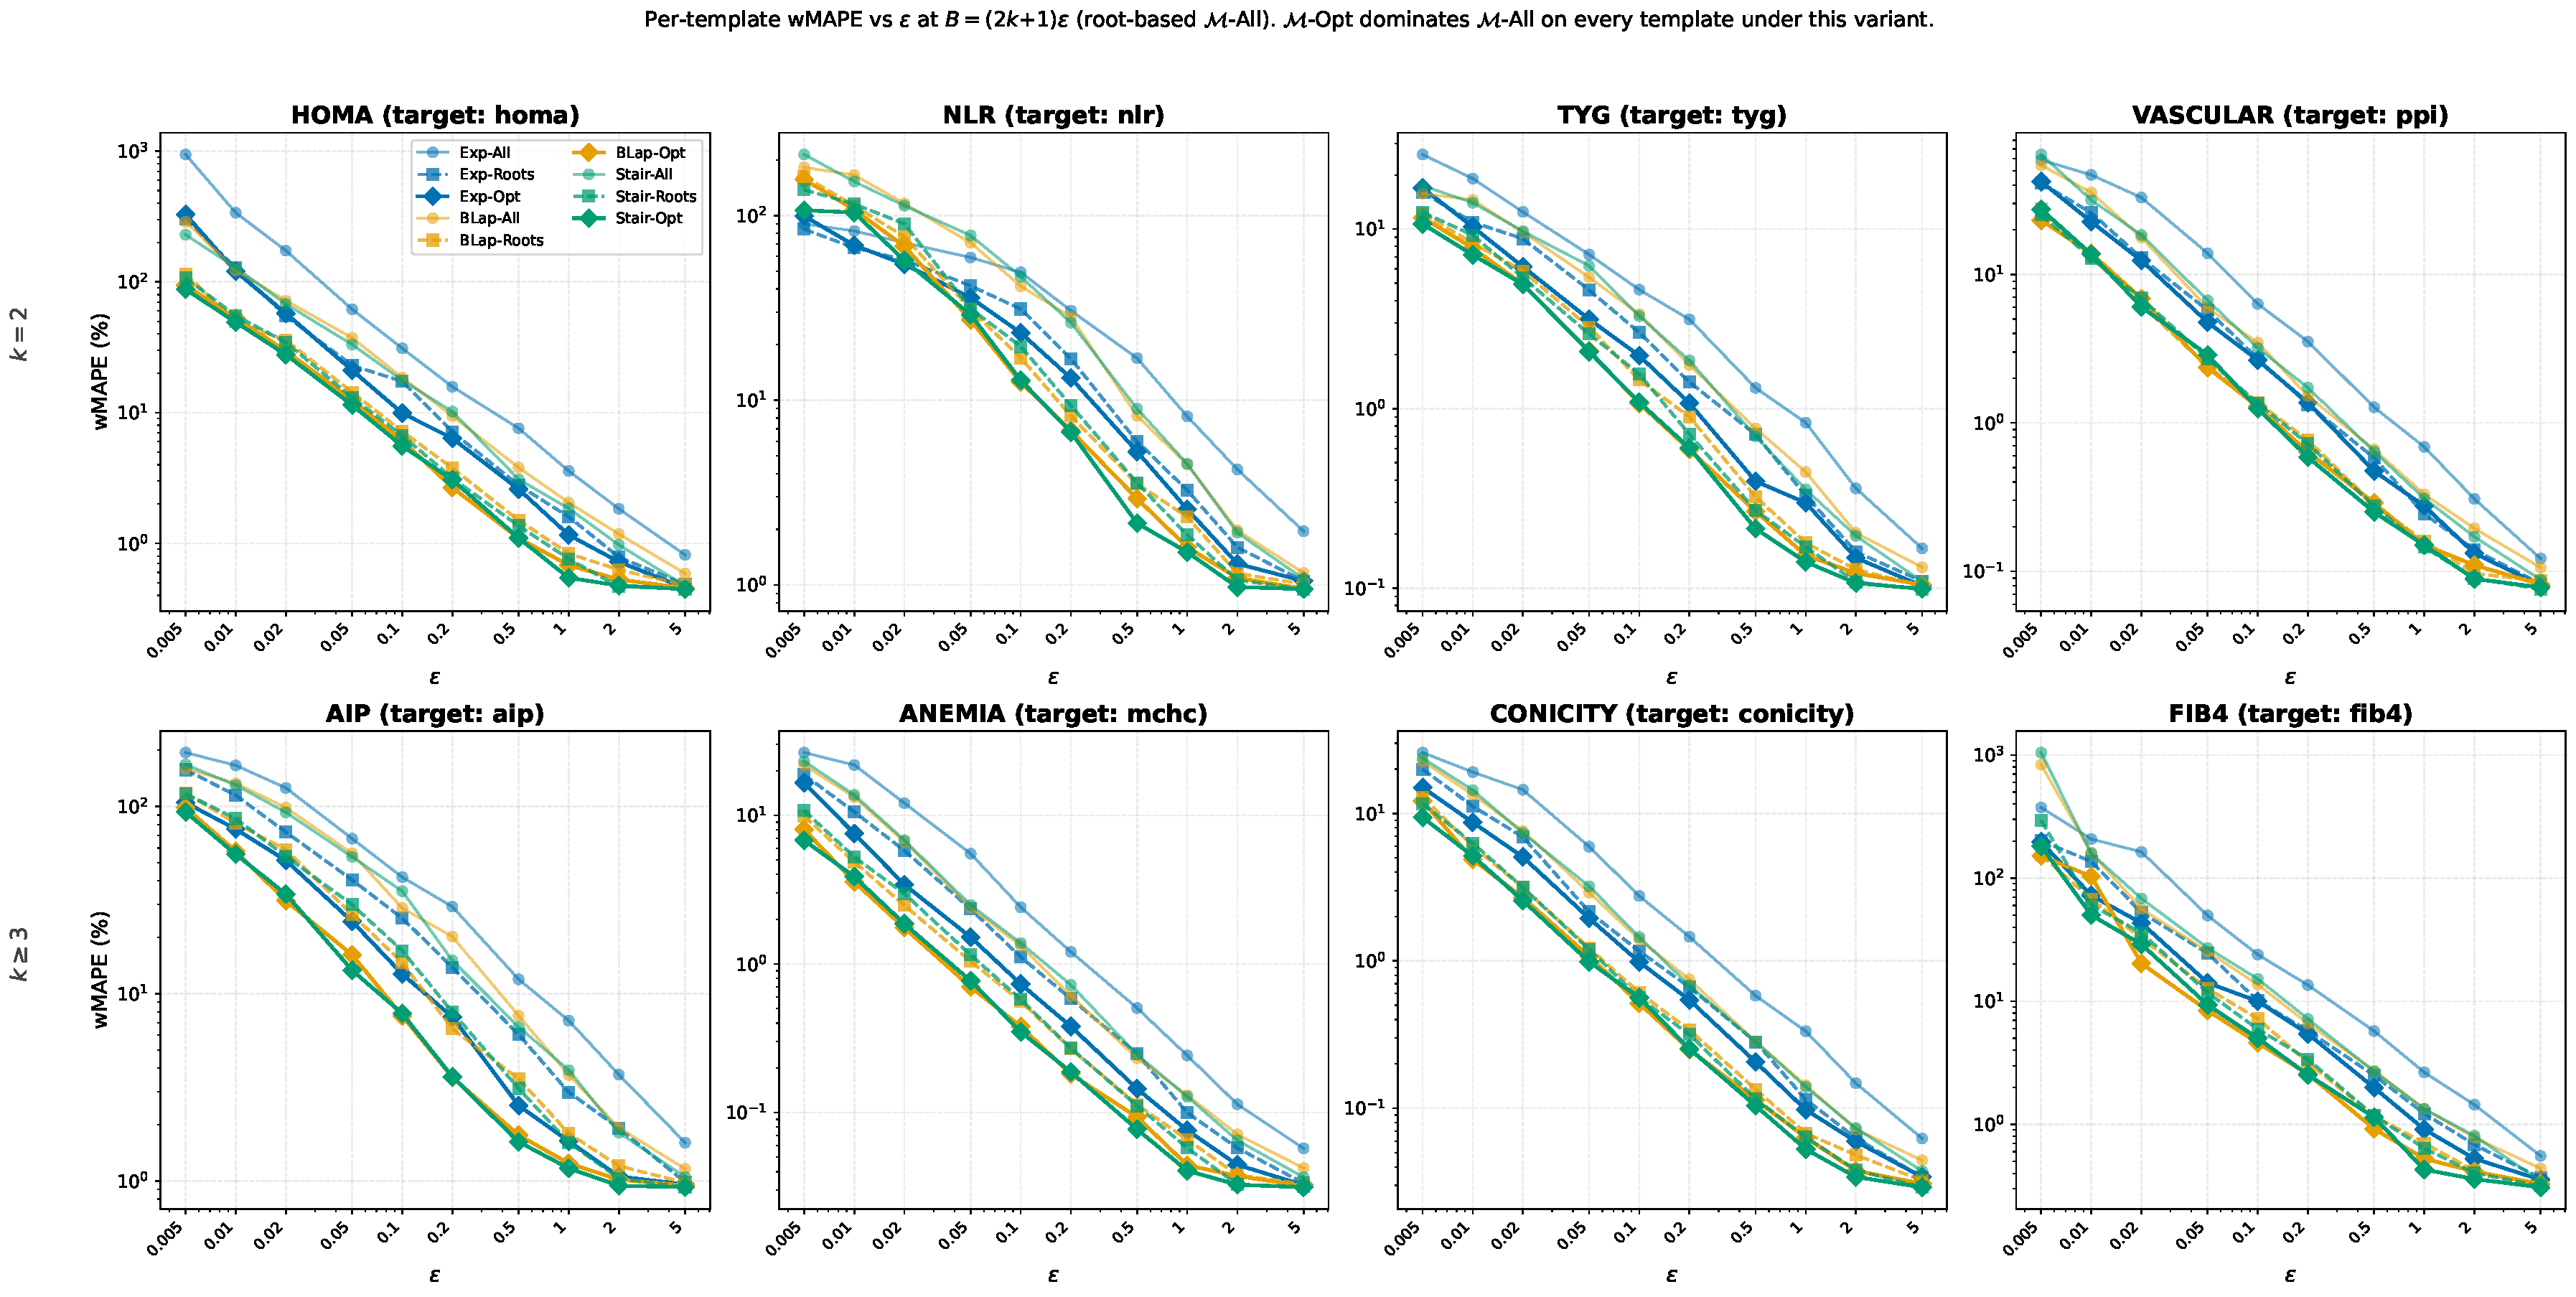
\includegraphics[width=\linewidth]{figures/rq1_per_template_grid.pdf}
    \caption{Per-template wMAPE (\%) vs.\ $\varepsilon$ at $B = (2k{+}1)\varepsilon$.
    Top row: compressing formulas with high-error baselines (FIB4, HOMA, AIP,
    NLR). Bottom row: amplifying formulas with already-low base errors (ANEMIA,
    CONICITY, TYG, VASCULAR). Nine methods per panel
    (3 mechanisms $\times$ 3 variants). The headline cell ($\varepsilon = 0.1$,
    Exponential) is summarized in main-text Table~\ref{tab:per_template_summary};
    full numerical tables follow in App.~\ref{app:rq1-tables}.}
    \label{fig:per_template_app}
\end{figure*}



\subsection{Per-root Budget Allocation}
\label{app:per-root-budget}
Figure~\ref{fig:allocation_bars} shows the per-root budget shares across templates, mechanisms, and privacy levels: $\mathcal{M}$-Opt allocates more budget to influential roots in every condition. Figures~\ref{fig:allocation_powerlaw_10} and~\ref{fig:allocation_powerlaw_01} confirm the closed-form prediction $\varepsilon_i \propto \sqrt{|h_i|\,\delta_i}$ (Sec.~\ref{sec:opt-budget}) on log-log axes for all three mechanisms at $\varepsilon = 0.1$ and $\varepsilon = 1.0$, with fitted slopes within $\pm 0.02$ of the predicted $0.5$.
% We show the per root budget allocation across different templates, mechanisms and privacy parameters in Figure~\ref{fig:allocation_bars}. All $\mathcal{M}$-Opt methods exploit the budget to minimize target node error, by allocating more budget to influential nodes. Figure~\ref{fig:allocation_powerlaw_01}---~\ref{fig:allocation_powerlaw_10} show the allocation following the power law, for $\varepsilon = 0.1$ and $\varepsilon = 1.0$ respectively.

\begin{figure*}[t]
\centering
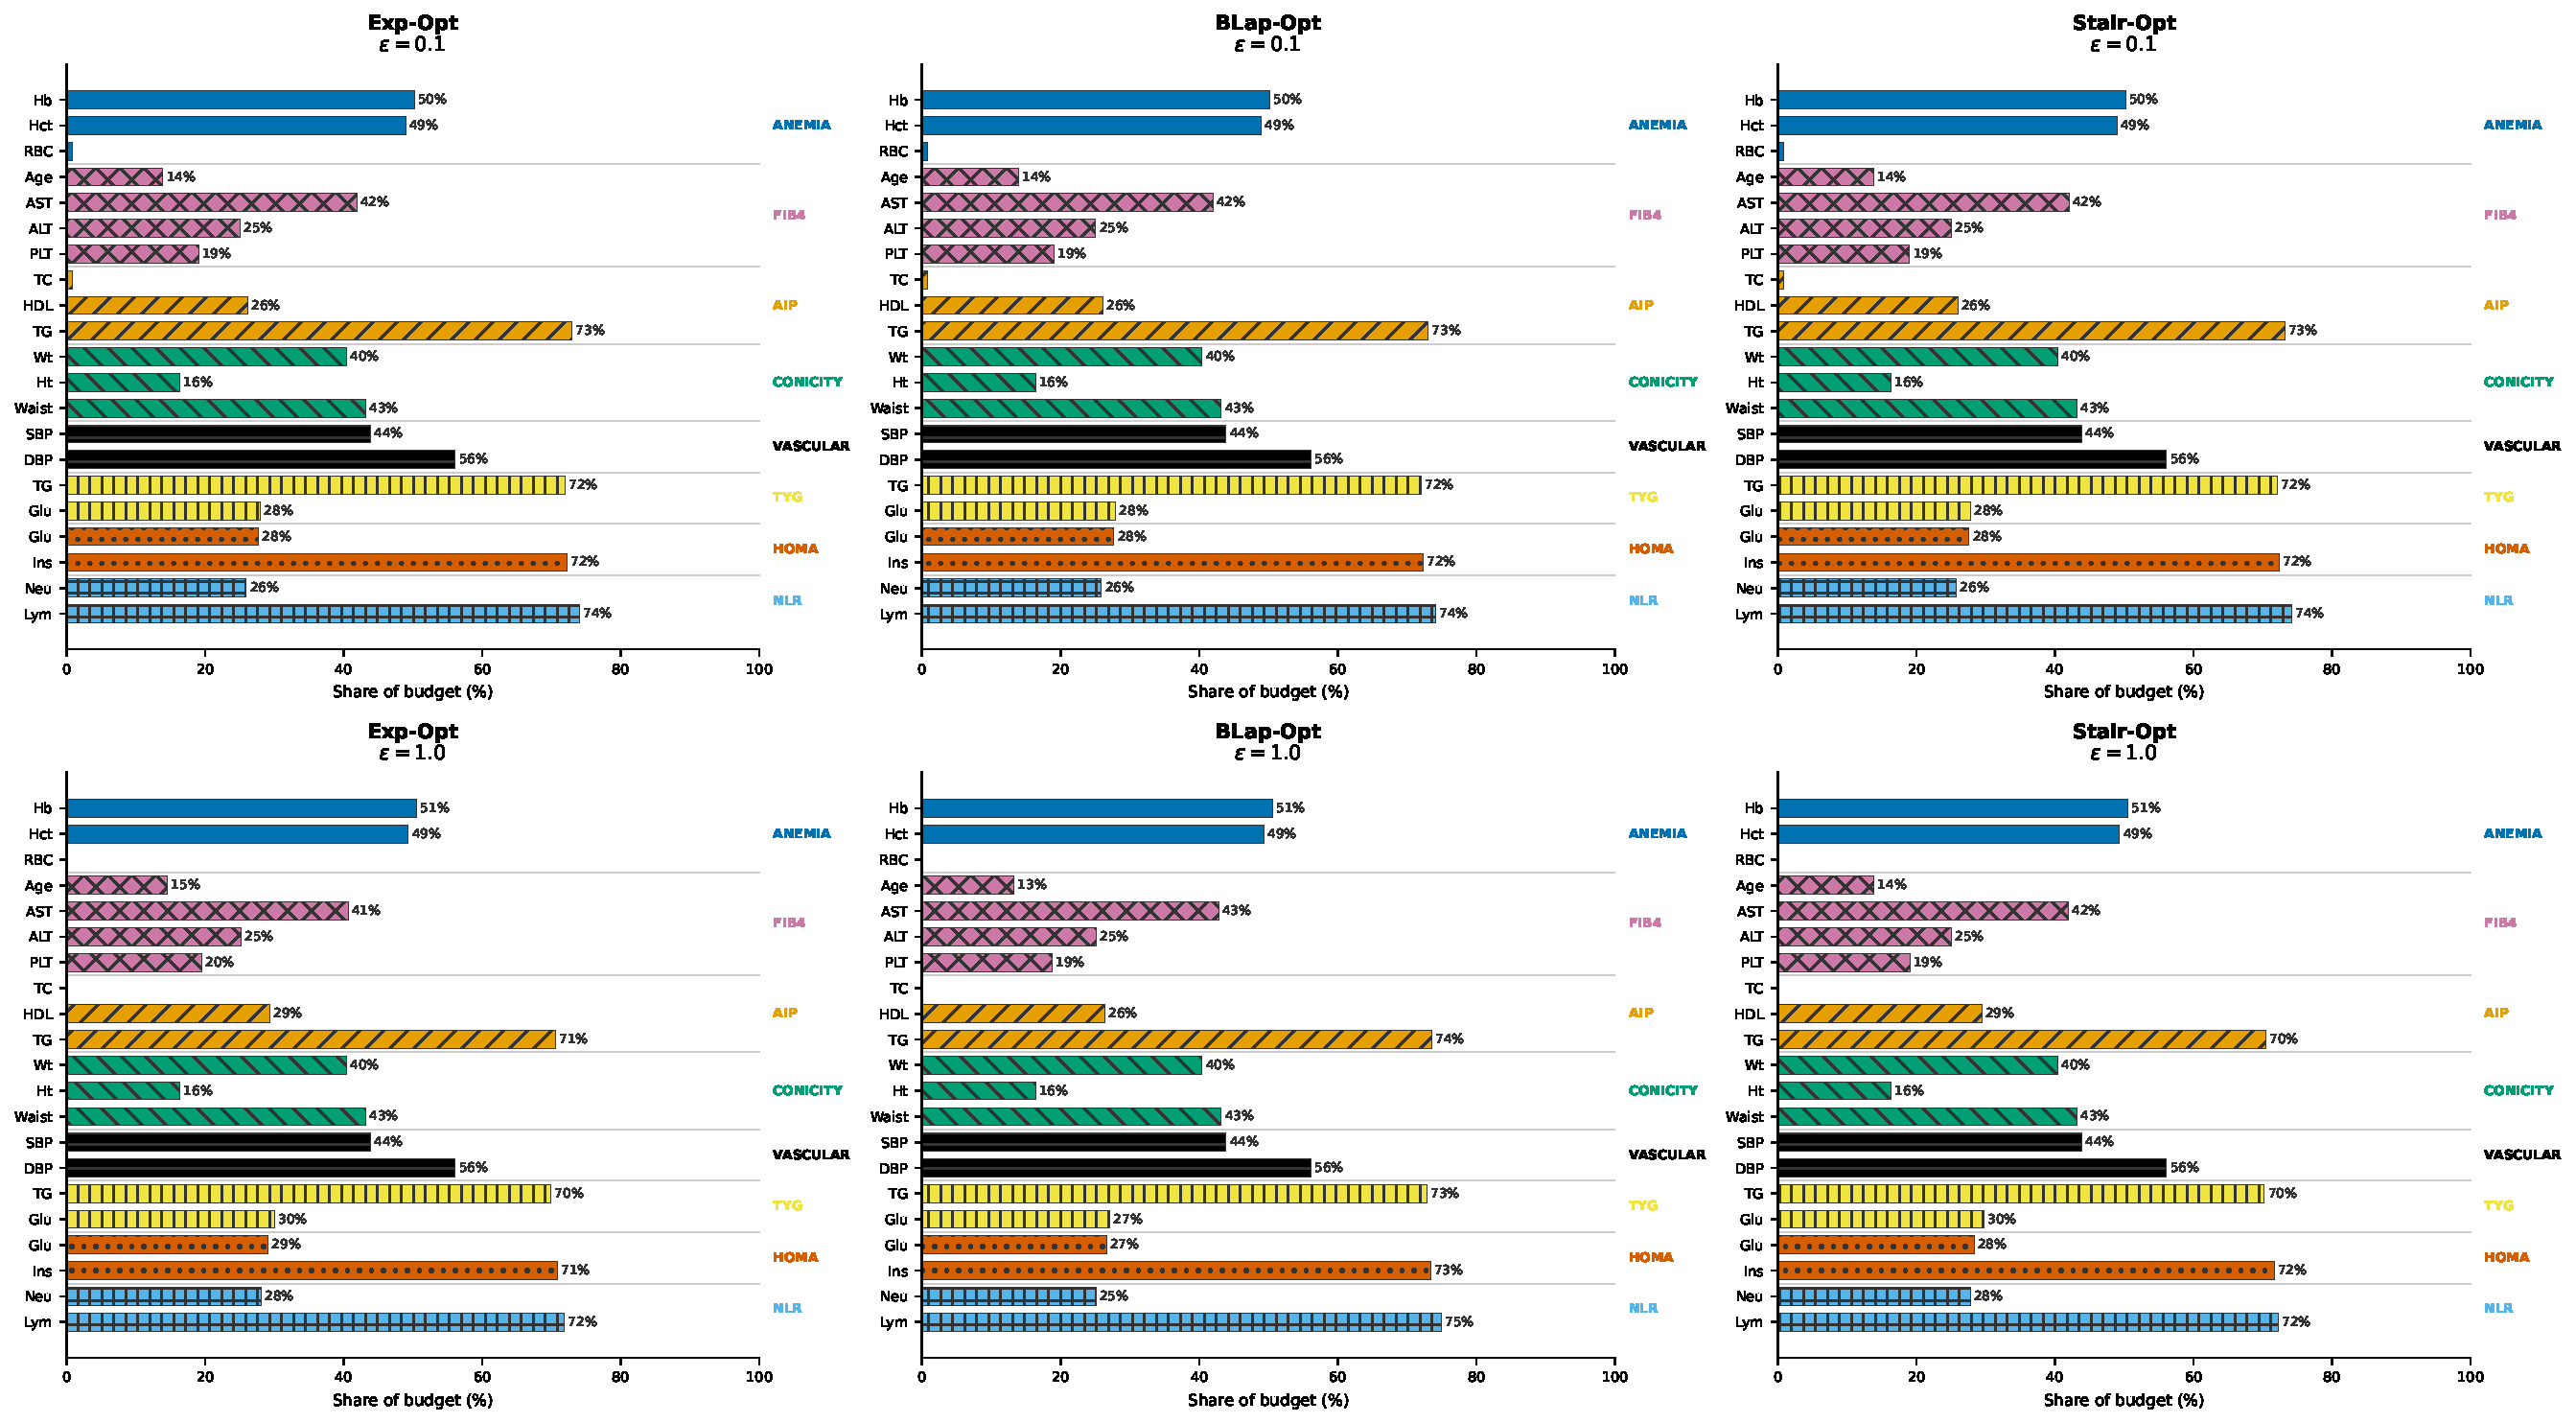
\includegraphics[width=\textwidth]{figures/rq2_allocation_by_mechanism.pdf}
\caption{Per-root budget shares (\%) for three mechanisms at $\varepsilon = 0.1$ (left three panels) and $\varepsilon = 1.0$ (right three).  Allocations are nearly identical across mechanisms at low $\varepsilon$; at $\varepsilon = 1.0$ minor mechanism-specific differences emerge (e.g., BLap assigns 43\% to AST in FIB4 vs.\ Exp's 41\%).}
\label{fig:allocation_bars}
\end{figure*}

\subsection{Closed-Form Budget Allocation in the Laplace Limit}
\label{app:budget-derivation}
 
Sec.~\ref{sec:opt-budget} establishes the optimization
\[
    \min_{\epsilon_1, \dots, \epsilon_k} \sum_{i=1}^k |h_i| \cdot \bar{\eta}_i(\epsilon_i)
    \qquad \text{s.t.} \qquad
    \sum_{i=1}^k \epsilon_i = B, \quad \epsilon_i \geq \epsilon_{\min}.
\]
The objective is solved numerically for each mechanism. Here we derive the closed-form solution in the Laplace limit, where the discrete index-space distribution of Sec.~\ref{sec:sanitization} converges to a continuous Laplace distribution as the grid becomes fine ($m \to \infty$).

\paragraph{Setup and bound.} Each root is independently sanitized via $\mathcal{M}_{\epsilon_i}$, producing output index $s$ and domain-unit noise $\eta_i = (s - t_i)\,\delta_i$. Let $x' = (x_1', \dots, x_k')$ be the sanitized vector with $x_i' = s\,\delta_i + \ell_i$. The error in the intermediate $g$ is $\Delta = g(x') - g(x)$; a first-order expansion gives $\Delta \approx \sum_{i=1}^{k} h_i\,\eta_i$. Applying the triangle inequality inside the expectation,
\begin{align*}
    \mathbb{E}\big[|\Delta|\big]
    \;\approx\; \mathbb{E}\Big[\Big|\sum_{i=1}^k h_i\,\eta_i\Big|\Big]
    \;\leq\; \sum_{i=1}^k |h_i|\,\mathbb{E}\big[|\eta_i|\big].
\end{align*}
Since the $\eta_i$ are independent (each mechanism uses independent randomness), this upper bound is tight up to cancellation effects. The expected absolute noise $\mathbb{E}[|\eta_i|]$ depends on $t_i$, the true value's position within the grid; to keep the optimization data-independent, we take the worst case over all positions:
\begin{equation}
\label{eq:bar-eta}
    \bar{\eta}_i(\epsilon_i) = \sup_{t_i \in [0,\, m-1]} \mathbb{E}\big[|\eta_i|\big].
\end{equation}
This yields the optimization restated above.
 
\paragraph{Continuum approximation.} For the discrete Exponential mechanism, the sampling weight at index $s$ is $P(s) \propto \exp(-\epsilon_i |t_i - s|/2)$. As $m \to \infty$, this converges to a Laplace distribution centered at $t_i$ with scale $b_i = 2/\epsilon_i$ in index units. The expected absolute deviation of a Laplace with scale $b_i$ is $b_i$. In domain units, $\bar{\eta}_i(\epsilon_i) \approx 2\delta_i / \epsilon_i$. The Bounded Laplace mechanism is asymptotically identical (truncation effects are exponentially small in $\epsilon_i (m{-}1)$).
 
\paragraph{Lagrangian.} Substituting into the objective, the Lagrangian for the active constraint set ($\epsilon_i > \epsilon_{\min}$) becomes
\begin{align*}
    \mathcal{L}(\epsilon_1, \dots, \epsilon_k, \lambda) = \sum_{i=1}^{k} |h_i|\,\frac{2\delta_i}{\epsilon_i} + \lambda\left(\sum_{i=1}^{k} \epsilon_i - B\right),
\end{align*}
where $\lambda \in \mathbb{R}$ is the multiplier for the budget constraint. Taking $\partial \mathcal{L}/\partial \epsilon_i = 0$,
\[
    -\frac{2|h_i|\,\delta_i}{\epsilon_i^2} + \lambda = 0
    \quad \Longrightarrow \quad
    \epsilon_i^* = \sqrt{\frac{2|h_i|\,\delta_i}{\lambda}}
    \;\propto\; \sqrt{|h_i|\,\delta_i}.
\]
Let $w_i = \sqrt{|h_i|\,\delta_i}$. Substituting $\epsilon_i^* = w_i \sqrt{2/\lambda}$ into the budget constraint $\sum_{i \in \mathcal{R}_A} \epsilon_i = B - |\mathcal{R}_S|\,\epsilon_{\min}$ (where $\mathcal{R}_A$ is the set of active roots and $\mathcal{R}_S$ is the set of saturated roots) and solving for $\lambda$ gives
\begin{equation}
\label{eq:closed-form}
    \tilde{\epsilon}_i = \frac{w_i}{\sum_{j \in \mathcal{R}_A} w_j} \left(B - |\mathcal{R}_S|\,\epsilon_{\min}\right).
\end{equation}
The second derivative of the objective, $4|h_i|\delta_i / \epsilon_i^3 > 0$ for all $\epsilon_i > 0$, confirms strict convexity, so this stationary point is the unique global minimum. This matches the closed-form claim made in Sec.~\ref{sec:opt-budget}.
 
\paragraph{Saturation handling.} We solve~\eqref{eq:closed-form} iteratively: roots whose allocation falls below $\epsilon_{\min}$ are clamped, removed from $\mathcal{R}_A$, added to $\mathcal{R}_S$, and the remaining budget is redistributed among the still-active roots. This terminates after at most $k$ iterations.
 
\paragraph{Discrete mechanisms.} For the discrete Exponential, Bounded Laplace, and Staircase mechanisms, we solve the optimization directly over the discrete $\bar{\eta}_i(\epsilon_i)$ via standard numerical optimization. RQ3 (Sec.~\ref{sec:experiments-rq3}) verifies that the scaling $\epsilon_i \propto \sqrt{|h_i| \delta_i}$ predicted by the Laplace closed-form holds empirically across all three discrete mechanisms (fitted log-log slope $0.50$ at $\varepsilon = 0.1$).
 
\paragraph{Sensitivity computation.} Sec.~\ref{sec:opt-budget} requires the sensitivity weights $h_i = |\partial g / \partial x_i(\mu)|$, evaluated at the population mean $\mu = (\mu_1, \dots, \mu_k)$. \sysname{} computes these via a single forward-mode automatic differentiation pass through the conversation DAG:
\begin{enumerate}
    \item Set all root values to their population means: $x = \mu$.
    \item Propagate values forward through the DAG in topological order, computing all intermediate node values.
    \item Propagate gradient seeds forward using the chain rule with exact analytical local partial derivatives at each node.
    \item Take absolute values: $h_i = |\partial g / \partial x_i(\mu)|$.
\end{enumerate}
Since target formulas may be nonlinear, $\partial g / \partial x_i$ can depend on the values of other roots; evaluating at $\mu$ captures these cross-dependencies at a representative operating point. The population means are domain knowledge --- in our experiments, computed from the NHANES~\cite{nhanes2017exam} reference population (excluding test data). If the deployment population differs substantially from the reference, the allocation may be suboptimal for that population, but the privacy guarantee remains $B$-mDP regardless: the weights $h_i$ enter the utility objective only and do not affect the privacy proof.

\subsection{Proof of Theorem~\ref{thm:privacy-guarantee}}
\label{app:thm:privacy-guarantee}

\begin{proof}[Proof of Theorem~\ref{thm:privacy-guarantee}]
By the privacy game definition,
\begin{align*}
\mathrm{Adv}_{\mathrm{DAG}}(\mathcal{A})
  &= |2\Pr[G_{\mathrm{DAG}}(\mathcal{A}) = 1] - 1| \\
  &= |\Pr[b'{=}0 \mid b{=}0] - \Pr[b'{=}0 \mid b{=}1]|.    
\end{align*}

The adversary's view in the game is fully determined by $\hat{X}^b$: $\mathcal{A}$ chooses $F$ at challenge time and computes $\hat{G}_b = C(\hat{X}^b, F)$ deterministically. Hence $\Pr[b'{=}0 \mid b]$ depends only on the distribution of $\hat{X}^b$ (and on $\mathcal{A}$'s fixed strategy on its view).

\medskip
\noindent\textbf{Hybrid argument.} Without loss of generality, assume $X^0$ and $X^1$ differ in exactly the roots $\{1, \ldots, k\}$. Define hybrids
\[
  X^{(0)} = X^0,\qquad X^{(j)} = (x^1_1, \ldots, x^1_j, x^0_{j+1}, \ldots, x^0_k),\qquad X^{(k)} = X^1.
\]
Each consecutive pair $(X^{(j-1)}, X^{(j)})$ differs in exactly root $j$. Let
\[
  p_j := \Pr[\mathcal{A}\text{ outputs } 0 \mid \text{input } X^{(j)}\text{ is sanitized}].
\]
Then $\Pr[b'{=}0 \mid b{=}0] = p_0$ and $\Pr[b'{=}0 \mid b{=}1] = p_k$, so
\[
  \mathrm{Adv}_{\mathrm{DAG}}(\mathcal{A}) = |p_0 - p_k|
  = \Big| \sum_{j=1}^{k} (p_{j-1} - p_j) \Big|
  \leq \sum_{j=1}^{k} |p_{j-1} - p_j|.
\]

\medskip
\noindent\textbf{Single-root step.} For each $j$, $X^{(j-1)}$ and $X^{(j)}$ agree everywhere except at root $j$ (where they take values $x^0_j$ and $x^1_j$ respectively), and the rest of the noised vector is sampled from the same distribution. Marginalizing over the shared roots, $|p_{j-1} - p_j|$ depends only on the distribution of the $j$-th sanitized component. Conditioning on the realized values of all other (shared) roots, denote
\[
  q_j(z) := \Pr[\mathcal{A}\text{ outputs } 0 \mid \text{root $j$ is sanitized to } z,\ \text{rest fixed to } X'^{(j)}].
\]
Then $|p_{j-1} - p_j| \leq \mathbb{E}_{X'^{(j)}}\big| \mathbb{E}_z[q_j(z) \mid x^0_j] - \mathbb{E}_z[q_j(z) \mid x^1_j] \big|$ where the inner expectations are over the noise of root $j$. We bound the inner difference for each fixed shared context.

\medskip
\noindent\textbf{Case 1: root $j$ is type $\tau_I$ (FPE).} By PRP security of FPE under security parameter $\kappa$, no polynomial-time adversary can distinguish $E_F(K, N_{\tau_j}, x^0_j)$ from $E_F(K, N_{\tau_j}, x^1_j)$ except with probability $\mathrm{negl}(\kappa)$. Hence
\[
  |p_{j-1} - p_j| \leq \mathrm{negl}(\kappa).
\]

\medskip
\noindent\textbf{Case 2: root $j$ is type $\tau_{II}$ (mDP with budget $\epsilon_j$).} The mechanism $M_{\epsilon_j}$ is $\epsilon_j$-mDP under the index-space metric $d(t, t') = |t - t'|$, with $|t_j^0 - t_j^1| = |x_j^0 - x_j^1| / \delta_j$. Hence for every measurable output set $S$,
\[
  \Pr[M_{\epsilon_j}(x_j^0) \in S] \leq e^{\epsilon_j |x_j^0 - x_j^1| / \delta_j} \Pr[M_{\epsilon_j}(x_j^1) \in S].
\]
Marginalizing $\mathcal{A}$'s output (a function of $\hat{X}^b$) over the noise distribution of root $j$ and applying this pointwise,
\begin{align*}
  \mathbb{E}_z[q_j(z) \mid x^0_j]
  &= \sum_z \Pr[M_{\epsilon_j}(x_j^0) = z]\, q_j(z) \\
  &\leq e^{\epsilon_j |x_j^0 - x_j^1| / \delta_j} \sum_z \Pr[M_{\epsilon_j}(x_j^1) = z]\, q_j(z) \\
  &= e^{\epsilon_j |x_j^0 - x_j^1| / \delta_j}\, \mathbb{E}_z[q_j(z) \mid x^1_j].
\end{align*}
Since each expectation is in $[0, 1]$, this gives
\[
  \big| \mathbb{E}_z[q_j(z) \mid x^0_j] - \mathbb{E}_z[q_j(z) \mid x^1_j] \big|
  \leq e^{\epsilon_j |x_j^0 - x_j^1| / \delta_j} - 1
  \leq e^{\epsilon_j |x_j^0 - x_j^1| / \delta_j}.
\]
Taking expectation over $X'^{(j)}$,
\[
  |p_{j-1} - p_j| \leq e^{\epsilon_j |x_j^0 - x_j^1| / \delta_j}.
\]

\medskip
\noindent\textbf{Combining.} Summing over $j$,
\[
  \mathrm{Adv}_{\mathrm{DAG}}(\mathcal{A})
  \leq \sum_{j \in [\tau_{II}]} e^{\epsilon_j |x_j^0 - x_j^1| / \delta_j} + |[\tau_I]| \cdot \mathrm{negl}(\kappa).
\]
\end{proof}

\subsection{Proof of Theorem~\ref{thm:privacy-leakage}}
\label{app:thm:privacy-leakage}
\begin{proof}
Since $\mathcal{M}$ is $\epsilon$-mDP on 
$(\mathcal{Y}, d_{\mathcal{Y}})$, for all 
$y, y' \in \mathcal{Y}$ and measurable 
$T \subseteq \mathcal{Y}$:
\[
    \Pr[\mathcal{M}(y) \in T] 
    \leq e^{\epsilon\, d_{\mathcal{Y}}(y, y')} 
    \Pr[\mathcal{M}(y') \in T].
\]
Let $y = f(x)$ and $y' = f(x')$ for some $x, x' \in \mathcal{X}$. Then:
\[
    \Pr[\mathcal{M}(f(x)) \in T] 
    \leq e^{\epsilon\, d_{\mathcal{Y}}(f(x), f(x'))} 
    \Pr[\mathcal{M}(f(x')) \in T].
\]
Apply the upper Lipschitz bound 
$d_{\mathcal{Y}}(f(x), f(x')) \leq L\, d_{\mathcal{X}}(x, x')$ and substitute $\psi$:
\[
    \Pr[\psi(x) \in T] 
    \leq e^{\epsilon\, L\, d_{\mathcal{X}}(x, x')} 
    \Pr[\psi(x') \in T].
\]
\end{proof}

% \subsection{Proof of Theorem~\ref{thm:total-leakage}}
% \label{app:thm:total-leakage}
% \begin{proof}
% Since all mechanisms use independent randomness, the joint density factors:
% \begin{align*}
%     &\prod_{r=1}^{k} \frac{\Pr[\mathcal{M}_r(x_r) \in S_r]}{\Pr[\mathcal{M}_r(x_r') \in S_r]} \cdot \prod_{j=1}^{d} \frac{\Pr[\mathcal{N}_j(f_j(x)) \in T_j]}{\Pr[\mathcal{N}_j(f_j(x')) \in T_j]}.
% \end{align*}
% Each root ratio is bounded by the $\epsilon_r$-mDP guarantee of $\mathcal{M}_r$:
% \[
%     \frac{\Pr[\mathcal{M}_r(x_r) \in S_r]}{\Pr[\mathcal{M}_r(x_r') \in S_r]} \leq e^{\epsilon_r\, |x_r - x_r'|}.`
% \]
% Each derived ratio is bounded by the $\hat{\epsilon}_j$-mDP guarantee of $\mathcal{N}_j$:
% \[
%     \frac{\Pr[\mathcal{N}_j(f_j(x)) \in T_j]}{\Pr[\mathcal{N}_j(f_j(x')) \in T_j]} \leq e^{\hat{\epsilon}_j\, |f_j(x) - f_j(x')|}.
% \]
% Taking the product yields the stated bound. For tightness: for each mechanism, there exists a choice of $S_r^*$ or $T_j^*$ that achieves the corresponding ratio. Since the mechanisms are independent, the product set $S_1^* \times \cdots \times S_k^* \times T_1^* \times \cdots \times T_d^*$ achieves all worst cases simultaneously.
% \end{proof}

\subsection{Proof of Theorem~\ref{thm:implied-privacy}}
\label{app:thm:implied-privacy}
\begin{proof}
Since $\mathcal{M}$ is an $\epsilon$-mDP mechanism on $(\mathcal{X}, d_\mathcal{X})$, 
\[
    \Pr[\mathcal{M}(x) \in S]
    \;\leq\;
    e^{\epsilon \, d_{\mathcal{X}}(x, x')}
    \Pr[\mathcal{M}(x') \in S],
\]
where the probability is taken over the randomness of $\mathcal{M}$. \\

\noindent Fix $x, x' \in \mathcal{X}$ and let $T \subseteq \mathcal{Y}$ be any measurable set.  
Define $S = f^{-1}(T) \subseteq \mathcal{X}$. \\

\noindent Then, by the definition of $\phi = f \circ \mathcal{M}$,
\[
    \Pr[\phi(x) \in T]
    \;=\;
    \Pr[f(\mathcal{M}(x)) \in T]
    \;=\;
    \Pr[\mathcal{M}(x) \in S].
\]
Applying the mDP property of $\mathcal{M}$ yields
\begin{align*}
    \Pr[\mathcal{M}(x) \in S]
    &\leq
    e^{\epsilon \, d_{\mathcal{X}}(x, x')}
    \Pr[\mathcal{M}(x') \in S] \\
    \Rightarrow \quad
    \Pr[\phi(x) \in T]
    &\leq
    e^{\epsilon \, d_{\mathcal{X}}(x, x')}
    \Pr[\phi(x') \in T].
\end{align*}

\noindent Since $f$ is bi-Lipschitz, we have
\[
    d_{\mathcal{X}}(x, x')
    \;\leq\;
    \frac{1}{\alpha} \, d_{\mathcal{Y}}(f(x), f(x')).
\]

\noindent Substituting this bound into the inequality above gives
\[
    \Pr[\phi(x) \in T]
    \;\leq\;
    e^{\frac{\epsilon}{\alpha} \, d_{\mathcal{Y}}(f(x), f(x'))}
    \Pr[\phi(x') \in T].
\]

\noindent Thus, $\phi$ is $\frac{\epsilon}{\alpha}$-mDP with respect to the metric $d_{\mathcal{Y}}(f(x), f(x'))$.  
Consequently, adding mDP noise directly to $y = f(x)$ in $(\mathcal{Y}, d_{\mathcal{Y}})$ with privacy parameter $\frac{\epsilon}{\alpha}$ provides at least as strong a privacy guarantee as first noising $x$ and then applying $f$.
\end{proof}

% \subsection{Per-Template Privacy-Utility  Analysis}
\label{app:fair-utility-details}
\subsection{RQ1: Full Adversarial Utility Tables}
\label{app:rq1-tables}

This appendix provides the complete aggregate wMAPE and Risk Class Error (RCE) tables for all three mechanisms (Exponential, Bounded Laplace, Staircase) under each of the three adversary turn budgets ($t \in \{k{+}1, 2k{+}1, 3k{+}1\}$). Per-template wMAPE breakdowns at $\varepsilon = 0.1$ are also included. The main text (Sec.~\ref{sec:experiments-rq1}) reports the Exponential mechanism; the Bounded Laplace and Staircase results follow the same trends. Bootstrap standard errors (1000 resamples) are shown inline as {\scriptsize $\pm$SE}; aggregate SEs are propagated from per-template SEs as $\sqrt{\sum_i \mathrm{SE}_i^2}/k$.

\begin{table*}[t]
\centering
\setlength{\tabcolsep}{2.8pt}
\small
\caption{Aggregate wMAPE (\%) averaged across 8 templates with bootstrap SE. Budget $B = (k+1) \cdot \varepsilon$. Best mean per row in \textbf{bold}.}
\label{tab:rq1_kplus1_wmape}
\begin{tabular}{cc|ccc|ccc|ccc}
\toprule
& & \multicolumn{3}{c|}{\textbf{Exponential}} & \multicolumn{3}{c|}{\textbf{Bounded Laplace}} & \multicolumn{3}{c}{\textbf{Staircase}} \\
$\varepsilon$ & $\bar{B}$ & All & Roots & Opt & All & Roots & Opt & All & Roots & Opt \\
\midrule
5.0 & 18.12 & 0.6\pmstd{0.0} & 0.5\pmstd{0.0} & 0.4\pmstd{0.0} & 0.5\pmstd{0.0} & 0.4\pmstd{0.0} & 0.4\pmstd{0.0} & 0.4\pmstd{0.0} & 0.4\pmstd{0.0} & \textbf{0.4\pmstd{0.0}} \\
2.0 & 7.25 & 1.4\pmstd{0.1} & 1.0\pmstd{0.1} & 0.7\pmstd{0.0} & 0.8\pmstd{0.0} & 0.7\pmstd{0.0} & 0.5\pmstd{0.0} & 0.8\pmstd{0.0} & 0.5\pmstd{0.0} & \textbf{0.4\pmstd{0.0}} \\
1.0 & 3.62 & 3.0\pmstd{0.2} & 2.0\pmstd{0.1} & 1.3\pmstd{0.1} & 1.6\pmstd{0.1} & 1.1\pmstd{0.1} & 0.8\pmstd{0.0} & 1.5\pmstd{0.1} & 1.0\pmstd{0.1} & \textbf{0.7\pmstd{0.0}} \\
0.5 & 1.81 & 5.6\pmstd{0.3} & 4.0\pmstd{0.2} & 2.7\pmstd{0.1} & 3.1\pmstd{0.2} & 2.2\pmstd{0.1} & \textbf{1.4\pmstd{0.1}} & 3.1\pmstd{0.2} & 2.1\pmstd{0.1} & 1.5\pmstd{0.1} \\
0.2 & 0.73 & 12.6\pmstd{0.6} & 10.1\pmstd{0.5} & 6.6\pmstd{0.3} & 7.7\pmstd{0.5} & 5.6\pmstd{0.3} & 3.7\pmstd{0.2} & 7.4\pmstd{0.4} & 5.3\pmstd{0.3} & \textbf{3.4\pmstd{0.2}} \\
0.1 & 0.36 & 20.5\pmstd{0.9} & 14.9\pmstd{0.7} & 13.6\pmstd{0.7} & 14.3\pmstd{0.7} & 10.2\pmstd{0.5} & 6.9\pmstd{0.4} & 14.8\pmstd{0.8} & 10.5\pmstd{0.6} & \textbf{6.9\pmstd{0.3}} \\
0.05 & 0.18 & 35.0\pmstd{1.4} & 26.0\pmstd{1.1} & 21.6\pmstd{0.9} & 25.8\pmstd{1.2} & 19.0\pmstd{1.0} & \textbf{14.6\pmstd{0.7}} & 26.9\pmstd{1.2} & 20.7\pmstd{1.0} & 15.4\pmstd{0.8} \\
0.02 & 0.07 & 70.3\pmstd{4.3} & 55.5\pmstd{6.8} & 46.0\pmstd{2.8} & 51.5\pmstd{2.4} & 39.1\pmstd{1.7} & \textbf{29.8\pmstd{1.3}} & 50.6\pmstd{2.3} & 38.5\pmstd{1.6} & 31.3\pmstd{1.3} \\
0.01 & 0.04 & 122\pmstd{10.1} & 102\pmstd{9.6} & 86.6\pmstd{6.2} & 118\pmstd{33.3} & 63.7\pmstd{3.1} & \textbf{56.5\pmstd{2.9}} & 90.4\pmstd{6.4} & 61.1\pmstd{3.4} & 57.6\pmstd{5.1} \\
0.005 & 0.02 & 218\pmstd{18.4} & 154\pmstd{11.7} & \textbf{120\pmstd{10.1}} & 202\pmstd{29.9} & 138\pmstd{21.7} & 161\pmstd{19.5} & 158\pmstd{25.8} & 122\pmstd{12.1} & 136\pmstd{19.7} \\
\bottomrule
\end{tabular}
\end{table*}

\begin{table*}[t]
\centering
\setlength{\tabcolsep}{2.8pt}
\small
\caption{Aggregate Risk Class Error (\%) averaged across 8 templates with bootstrap SE. Budget $B = (k+1) \cdot \varepsilon$. Best mean per row in \textbf{bold}.}
\label{tab:rq1_kplus1_rce}
\begin{tabular}{cc|ccc|ccc|ccc}
\toprule
& & \multicolumn{3}{c|}{\textbf{Exponential}} & \multicolumn{3}{c|}{\textbf{Bounded Laplace}} & \multicolumn{3}{c}{\textbf{Staircase}} \\
$\varepsilon$ & $\bar{B}$ & All & Roots & Opt & All & Roots & Opt & All & Roots & Opt \\
\midrule
5.0 & 18.12 & 0.7\pmstd{0.2} & 0.6\pmstd{0.2} & \textbf{0.4\pmstd{0.2}} & 0.5\pmstd{0.2} & 0.5\pmstd{0.2} & 0.6\pmstd{0.2} & 0.6\pmstd{0.2} & 0.4\pmstd{0.2} & 0.4\pmstd{0.2} \\
2.0 & 7.25 & 1.6\pmstd{0.3} & 1.2\pmstd{0.3} & 0.6\pmstd{0.2} & 1.0\pmstd{0.2} & 0.9\pmstd{0.2} & 0.7\pmstd{0.2} & 1.0\pmstd{0.2} & 1.1\pmstd{0.3} & \textbf{0.5\pmstd{0.2}} \\
1.0 & 3.62 & 2.9\pmstd{0.4} & 2.1\pmstd{0.3} & 1.4\pmstd{0.3} & 1.7\pmstd{0.3} & 0.9\pmstd{0.2} & 0.8\pmstd{0.2} & 1.5\pmstd{0.3} & \textbf{0.7\pmstd{0.2}} & 0.9\pmstd{0.2} \\
0.5 & 1.81 & 5.1\pmstd{0.5} & 3.2\pmstd{0.4} & 2.8\pmstd{0.4} & 3.0\pmstd{0.4} & 2.2\pmstd{0.4} & 1.5\pmstd{0.3} & 3.3\pmstd{0.4} & 2.0\pmstd{0.3} & \textbf{1.4\pmstd{0.3}} \\
0.2 & 0.73 & 11.2\pmstd{0.7} & 8.6\pmstd{0.7} & 5.8\pmstd{0.5} & 5.9\pmstd{0.6} & 4.4\pmstd{0.5} & 3.5\pmstd{0.4} & 5.5\pmstd{0.5} & 4.6\pmstd{0.5} & \textbf{3.4\pmstd{0.4}} \\
0.1 & 0.36 & 15.4\pmstd{0.9} & 12.4\pmstd{0.7} & 10.3\pmstd{0.7} & 11.5\pmstd{0.7} & 8.5\pmstd{0.6} & 6.2\pmstd{0.6} & 10.3\pmstd{0.7} & 7.8\pmstd{0.6} & \textbf{5.2\pmstd{0.5}} \\
0.05 & 0.18 & 24.2\pmstd{1.0} & 19.1\pmstd{0.9} & 16.5\pmstd{0.9} & 19.3\pmstd{0.9} & 13.7\pmstd{0.8} & 11.5\pmstd{0.7} & 18.3\pmstd{0.9} & 14.2\pmstd{0.8} & \textbf{11.0\pmstd{0.7}} \\
0.02 & 0.07 & 32.3\pmstd{1.1} & 29.6\pmstd{1.1} & 26.0\pmstd{1.0} & 29.4\pmstd{1.1} & 26.3\pmstd{1.1} & \textbf{18.8\pmstd{0.9}} & 29.5\pmstd{1.1} & 24.9\pmstd{1.0} & 19.5\pmstd{0.9} \\
0.01 & 0.04 & 36.7\pmstd{1.1} & 34.4\pmstd{1.1} & 34.6\pmstd{1.1} & 37.4\pmstd{1.2} & 34.2\pmstd{1.1} & 30.0\pmstd{1.1} & 38.2\pmstd{1.2} & 33.8\pmstd{1.1} & \textbf{28.6\pmstd{1.1}} \\
0.005 & 0.02 & 38.3\pmstd{1.2} & 38.8\pmstd{1.1} & 37.9\pmstd{1.2} & 46.1\pmstd{1.2} & 41.5\pmstd{1.2} & 40.4\pmstd{1.2} & 44.3\pmstd{1.2} & 41.9\pmstd{1.2} & \textbf{37.6\pmstd{1.2}} \\
\bottomrule
\end{tabular}
\end{table*}

\begin{table*}[t]
\centering
\setlength{\tabcolsep}{2.8pt}
\small
\caption{Per-template wMAPE (\%) with bootstrap SE at $\varepsilon = 0.1$ ($\bar{B} = 0.36$). Budget $B = (k+1) \cdot \varepsilon$. Best per row in \textbf{bold}.}
\label{tab:rq1_kplus1_per_tmpl_wmape}
\begin{tabular}{l|ccc|ccc|ccc}
\toprule
& \multicolumn{3}{c|}{\textbf{Exponential}} & \multicolumn{3}{c|}{\textbf{Bounded Laplace}} & \multicolumn{3}{c}{\textbf{Staircase}} \\
Template & All & Roots & Opt & All & Roots & Opt & All & Roots & Opt \\
\midrule
ANEMIA & 2.6\pmstd{0.2} & 1.9\pmstd{0.1} & 1.2\pmstd{0.1} & 1.4\pmstd{0.1} & 0.9\pmstd{0.1} & 0.7\pmstd{0.1} & 1.2\pmstd{0.1} & 0.9\pmstd{0.1} & \textbf{0.6\pmstd{0.0}} \\
FIB4 & 25.3\pmstd{2.4} & 21.4\pmstd{2.1} & 17.8\pmstd{2.2} & 14.3\pmstd{1.4} & 11.0\pmstd{0.9} & \textbf{8.0\pmstd{0.7}} & 15.1\pmstd{2.0} & 9.8\pmstd{0.8} & 8.8\pmstd{0.8} \\
AIP & 43.8\pmstd{4.2} & 33.8\pmstd{3.3} & 25.3\pmstd{2.5} & 30.7\pmstd{3.3} & 23.5\pmstd{2.5} & 12.7\pmstd{1.3} & 29.1\pmstd{3.1} & 25.1\pmstd{2.7} & \textbf{12.0\pmstd{1.3}} \\
CONICITY & 2.6\pmstd{0.2} & 2.4\pmstd{0.1} & 1.8\pmstd{0.1} & 1.5\pmstd{0.1} & 0.9\pmstd{0.1} & 0.9\pmstd{0.1} & 1.5\pmstd{0.1} & 1.0\pmstd{0.1} & \textbf{0.9\pmstd{0.1}} \\
VASCULAR & 6.6\pmstd{0.5} & 4.4\pmstd{0.3} & 4.4\pmstd{0.3} & 3.3\pmstd{0.3} & 2.2\pmstd{0.2} & 2.4\pmstd{0.2} & 3.5\pmstd{0.3} & 2.1\pmstd{0.2} & \textbf{2.1\pmstd{0.1}} \\
TYG & 4.5\pmstd{0.3} & 3.4\pmstd{0.2} & 3.1\pmstd{0.2} & 3.5\pmstd{0.3} & 2.3\pmstd{0.2} & \textbf{1.7\pmstd{0.1}} & 3.2\pmstd{0.2} & 2.2\pmstd{0.2} & 1.8\pmstd{0.2} \\
HOMA & 28.5\pmstd{3.6} & 19.0\pmstd{2.8} & 18.1\pmstd{2.4} & 18.9\pmstd{2.2} & 12.3\pmstd{1.6} & \textbf{9.9\pmstd{1.3}} & 18.9\pmstd{2.3} & 12.2\pmstd{1.8} & 11.1\pmstd{1.0} \\
NLR & 49.8\pmstd{3.7} & 32.8\pmstd{2.4} & 37.5\pmstd{3.2} & 40.8\pmstd{3.8} & 28.2\pmstd{3.0} & 19.0\pmstd{2.0} & 46.1\pmstd{4.7} & 30.4\pmstd{3.0} & \textbf{18.1\pmstd{1.7}} \\
\bottomrule
\end{tabular}
\end{table*}

\begin{table*}[t]
\centering
\setlength{\tabcolsep}{2.8pt}
\small
\caption{Aggregate wMAPE (\%) averaged across 8 templates with bootstrap SE. Budget $B = (2k+1) \cdot \varepsilon$. Best mean per row in \textbf{bold}.}
\label{tab:rq1_2kplus1_wmape}
\begin{tabular}{cc|ccc|ccc|ccc}
\toprule
& & \multicolumn{3}{c|}{\textbf{Exponential}} & \multicolumn{3}{c|}{\textbf{Bounded Laplace}} & \multicolumn{3}{c}{\textbf{Staircase}} \\
$\varepsilon$ & $\bar{B}$ & All & Roots & Opt & All & Roots & Opt & All & Roots & Opt \\
\midrule
5.0 & 31.25 & 0.7\pmstd{0.0} & 0.4\pmstd{0.0} & 0.4\pmstd{0.0} & 0.5\pmstd{0.0} & 0.4\pmstd{0.0} & 0.4\pmstd{0.0} & 0.4\pmstd{0.0} & 0.4\pmstd{0.0} & \textbf{0.4\pmstd{0.0}} \\
2.0 & 12.50 & 1.5\pmstd{0.1} & 0.7\pmstd{0.0} & 0.5\pmstd{0.0} & 0.8\pmstd{0.0} & 0.5\pmstd{0.0} & 0.4\pmstd{0.0} & 0.8\pmstd{0.0} & 0.4\pmstd{0.0} & \textbf{0.4\pmstd{0.0}} \\
1.0 & 6.25 & 3.0\pmstd{0.2} & 1.2\pmstd{0.1} & 0.9\pmstd{0.1} & 1.6\pmstd{0.1} & 0.8\pmstd{0.0} & 0.6\pmstd{0.0} & 1.6\pmstd{0.1} & 0.7\pmstd{0.0} & \textbf{0.5\pmstd{0.0}} \\
0.5 & 3.12 & 5.7\pmstd{0.3} & 2.4\pmstd{0.1} & 1.7\pmstd{0.1} & 3.0\pmstd{0.2} & 1.3\pmstd{0.1} & 0.9\pmstd{0.0} & 2.9\pmstd{0.2} & 1.2\pmstd{0.1} & \textbf{0.8\pmstd{0.0}} \\
0.2 & 1.25 & 12.3\pmstd{0.6} & 5.9\pmstd{0.4} & 4.5\pmstd{0.2} & 8.6\pmstd{0.5} & 3.0\pmstd{0.2} & \textbf{2.2\pmstd{0.1}} & 8.0\pmstd{0.5} & 3.2\pmstd{0.2} & 2.2\pmstd{0.1} \\
0.1 & 0.62 & 20.3\pmstd{1.0} & 11.4\pmstd{0.6} & 7.8\pmstd{0.3} & 14.0\pmstd{0.8} & 6.2\pmstd{0.4} & \textbf{4.3\pmstd{0.3}} & 15.5\pmstd{0.8} & 6.6\pmstd{0.4} & 4.3\pmstd{0.2} \\
0.05 & 0.31 & 33.8\pmstd{1.7} & 18.0\pmstd{0.8} & 13.3\pmstd{0.6} & 25.8\pmstd{1.3} & 11.5\pmstd{0.6} & 8.8\pmstd{0.5} & 26.3\pmstd{1.2} & 11.7\pmstd{0.6} & \textbf{8.7\pmstd{0.4}} \\
0.02 & 0.12 & 75.7\pmstd{10.9} & 34.1\pmstd{1.5} & 29.2\pmstd{1.2} & 48.1\pmstd{2.0} & 27.7\pmstd{1.3} & 20.7\pmstd{1.0} & 48.0\pmstd{2.1} & 29.1\pmstd{1.3} & \textbf{20.4\pmstd{1.0}} \\
0.01 & 0.06 & 113\pmstd{8.4} & 63.0\pmstd{5.4} & 48.3\pmstd{2.6} & 82.4\pmstd{3.9} & 43.0\pmstd{1.8} & 43.9\pmstd{5.8} & 80.4\pmstd{5.4} & 43.9\pmstd{2.0} & \textbf{36.1\pmstd{1.7}} \\
0.005 & 0.03 & 218\pmstd{20.7} & 105\pmstd{6.9} & 102\pmstd{6.8} & 198\pmstd{27.5} & 76.5\pmstd{4.2} & 69.5\pmstd{5.2} & 223\pmstd{44.9} & 89.4\pmstd{13.8} & \textbf{65.5\pmstd{4.6}} \\
\bottomrule
\end{tabular}
\end{table*}

\begin{table*}[t]
\centering
\setlength{\tabcolsep}{2.8pt}
\small
\caption{Aggregate Risk Class Error (\%) averaged across 8 templates with bootstrap SE. Budget $B = (2k+1) \cdot \varepsilon$. Best mean per row in \textbf{bold}.}
\label{tab:rq1_2kplus1_rce}
\begin{tabular}{cc|ccc|ccc|ccc}
\toprule
& & \multicolumn{3}{c|}{\textbf{Exponential}} & \multicolumn{3}{c|}{\textbf{Bounded Laplace}} & \multicolumn{3}{c}{\textbf{Staircase}} \\
$\varepsilon$ & $\bar{B}$ & All & Roots & Opt & All & Roots & Opt & All & Roots & Opt \\
\midrule
5.0 & 31.25 & 0.6\pmstd{0.2} & 0.5\pmstd{0.2} & 0.6\pmstd{0.2} & 0.7\pmstd{0.2} & 0.5\pmstd{0.2} & \textbf{0.3\pmstd{0.1}} & 0.5\pmstd{0.2} & 0.4\pmstd{0.2} & 0.4\pmstd{0.2} \\
2.0 & 12.50 & 1.7\pmstd{0.3} & 0.9\pmstd{0.2} & 0.9\pmstd{0.2} & 1.1\pmstd{0.2} & 0.5\pmstd{0.2} & 0.4\pmstd{0.2} & 0.8\pmstd{0.2} & 0.5\pmstd{0.2} & \textbf{0.3\pmstd{0.1}} \\
1.0 & 6.25 & 2.7\pmstd{0.4} & 1.5\pmstd{0.3} & 0.8\pmstd{0.2} & 1.9\pmstd{0.3} & 0.6\pmstd{0.2} & 0.9\pmstd{0.2} & 1.4\pmstd{0.3} & 0.9\pmstd{0.2} & \textbf{0.4\pmstd{0.2}} \\
0.5 & 3.12 & 4.8\pmstd{0.5} & 2.8\pmstd{0.4} & 1.9\pmstd{0.3} & 2.8\pmstd{0.4} & 1.3\pmstd{0.3} & 1.2\pmstd{0.3} & 2.9\pmstd{0.4} & 1.0\pmstd{0.2} & \textbf{0.9\pmstd{0.2}} \\
0.2 & 1.25 & 10.2\pmstd{0.7} & 4.6\pmstd{0.5} & 4.5\pmstd{0.5} & 6.2\pmstd{0.6} & 3.0\pmstd{0.4} & \textbf{2.2\pmstd{0.4}} & 6.6\pmstd{0.6} & 2.8\pmstd{0.4} & 2.4\pmstd{0.4} \\
0.1 & 0.62 & 15.7\pmstd{0.8} & 10.1\pmstd{0.7} & 7.0\pmstd{0.6} & 10.6\pmstd{0.7} & 5.4\pmstd{0.5} & 4.4\pmstd{0.5} & 11.5\pmstd{0.7} & 5.4\pmstd{0.5} & \textbf{3.6\pmstd{0.4}} \\
0.05 & 0.31 & 23.2\pmstd{1.0} & 14.5\pmstd{0.8} & 11.7\pmstd{0.7} & 18.3\pmstd{0.9} & 9.2\pmstd{0.7} & 7.4\pmstd{0.6} & 19.5\pmstd{1.0} & 8.7\pmstd{0.7} & \textbf{6.4\pmstd{0.6}} \\
0.02 & 0.12 & 32.0\pmstd{1.1} & 25.4\pmstd{1.0} & 21.8\pmstd{1.0} & 30.2\pmstd{1.1} & 18.0\pmstd{0.9} & 14.8\pmstd{0.8} & 29.4\pmstd{1.1} & 20.4\pmstd{0.9} & \textbf{14.6\pmstd{0.8}} \\
0.01 & 0.06 & 35.8\pmstd{1.1} & 30.1\pmstd{1.1} & 27.2\pmstd{1.0} & 37.0\pmstd{1.2} & 27.1\pmstd{1.1} & 24.0\pmstd{1.0} & 37.8\pmstd{1.2} & 25.9\pmstd{1.1} & \textbf{23.1\pmstd{1.0}} \\
0.005 & 0.03 & 38.0\pmstd{1.1} & 34.6\pmstd{1.1} & 35.7\pmstd{1.1} & 42.5\pmstd{1.2} & 34.8\pmstd{1.2} & 33.6\pmstd{1.2} & 42.4\pmstd{1.2} & 35.1\pmstd{1.2} & \textbf{30.7\pmstd{1.1}} \\
\bottomrule
\end{tabular}
\end{table*}

\begin{table*}[t]
\centering
\setlength{\tabcolsep}{2.8pt}
\small
\caption{Per-template wMAPE (\%) with bootstrap SE at $\varepsilon = 0.1$ ($\bar{B} = 0.62$). Budget $B = (2k+1) \cdot \varepsilon$. Best per row in \textbf{bold}.}
\label{tab:rq1_2kplus1_per_tmpl_wmape}
\begin{tabular}{l|ccc|ccc|ccc}
\toprule
& \multicolumn{3}{c|}{\textbf{Exponential}} & \multicolumn{3}{c|}{\textbf{Bounded Laplace}} & \multicolumn{3}{c}{\textbf{Staircase}} \\
Template & All & Roots & Opt & All & Roots & Opt & All & Roots & Opt \\
\midrule
ANEMIA & 2.4\pmstd{0.1} & 1.1\pmstd{0.1} & 0.7\pmstd{0.0} & 1.3\pmstd{0.1} & 0.6\pmstd{0.0} & 0.4\pmstd{0.0} & 1.4\pmstd{0.1} & 0.6\pmstd{0.0} & \textbf{0.3\pmstd{0.0}} \\
FIB4 & 23.9\pmstd{1.8} & 10.1\pmstd{0.8} & 10.0\pmstd{0.9} & 13.7\pmstd{1.2} & 7.2\pmstd{0.7} & \textbf{4.6\pmstd{0.4}} & 15.2\pmstd{1.2} & 5.9\pmstd{0.5} & 5.0\pmstd{0.4} \\
AIP & 41.9\pmstd{4.1} & 25.3\pmstd{2.4} & 12.7\pmstd{1.4} & 28.7\pmstd{3.1} & 14.6\pmstd{1.6} & \textbf{7.6\pmstd{0.8}} & 35.3\pmstd{3.9} & 17.0\pmstd{2.0} & 7.8\pmstd{1.0} \\
CONICITY & 2.8\pmstd{0.2} & 1.2\pmstd{0.1} & 1.0\pmstd{0.1} & 1.4\pmstd{0.1} & 0.6\pmstd{0.0} & \textbf{0.5\pmstd{0.0}} & 1.5\pmstd{0.1} & 0.6\pmstd{0.0} & 0.6\pmstd{0.0} \\
VASCULAR & 6.3\pmstd{0.5} & 2.7\pmstd{0.2} & 2.6\pmstd{0.2} & 3.5\pmstd{0.2} & 1.4\pmstd{0.1} & 1.3\pmstd{0.1} & 3.2\pmstd{0.2} & 1.4\pmstd{0.1} & \textbf{1.2\pmstd{0.1}} \\
TYG & 4.6\pmstd{0.3} & 2.6\pmstd{0.2} & 2.0\pmstd{0.1} & 3.4\pmstd{0.3} & 1.4\pmstd{0.1} & \textbf{1.1\pmstd{0.1}} & 3.3\pmstd{0.3} & 1.6\pmstd{0.1} & 1.1\pmstd{0.1} \\
HOMA & 31.1\pmstd{4.4} & 17.3\pmstd{1.7} & 9.9\pmstd{1.2} & 18.5\pmstd{2.6} & 7.2\pmstd{1.0} & 6.1\pmstd{0.9} & 17.7\pmstd{2.3} & 6.7\pmstd{1.0} & \textbf{5.6\pmstd{0.7}} \\
NLR & 49.2\pmstd{4.3} & 31.2\pmstd{3.4} & 23.1\pmstd{1.5} & 41.4\pmstd{4.9} & 16.9\pmstd{2.0} & \textbf{12.5\pmstd{1.6}} & 46.6\pmstd{3.9} & 19.5\pmstd{2.6} & 12.8\pmstd{1.1} \\
\bottomrule
\end{tabular}
\end{table*}

\begin{table*}[t]
\centering
\setlength{\tabcolsep}{2.8pt}
\small
\caption{Aggregate wMAPE (\%) averaged across 8 templates with bootstrap SE. Budget $B = (3k+1) \cdot \varepsilon$. Best mean per row in \textbf{bold}.}
\label{tab:rq1_3kplus1_wmape}
\begin{tabular}{cc|ccc|ccc|ccc}
\toprule
& & \multicolumn{3}{c|}{\textbf{Exponential}} & \multicolumn{3}{c|}{\textbf{Bounded Laplace}} & \multicolumn{3}{c}{\textbf{Staircase}} \\
$\varepsilon$ & $\bar{B}$ & All & Roots & Opt & All & Roots & Opt & All & Roots & Opt \\
\midrule
5.0 & 44.38 & 0.6\pmstd{0.0} & 0.4\pmstd{0.0} & 0.4\pmstd{0.0} & 0.5\pmstd{0.0} & 0.4\pmstd{0.0} & 0.4\pmstd{0.0} & 0.4\pmstd{0.0} & \textbf{0.4\pmstd{0.0}} & 0.4\pmstd{0.0} \\
2.0 & 17.75 & 1.5\pmstd{0.1} & 0.5\pmstd{0.0} & 0.4\pmstd{0.0} & 0.8\pmstd{0.0} & 0.4\pmstd{0.0} & 0.4\pmstd{0.0} & 0.8\pmstd{0.1} & 0.4\pmstd{0.0} & \textbf{0.4\pmstd{0.0}} \\
1.0 & 8.88 & 3.0\pmstd{0.2} & 0.9\pmstd{0.1} & 0.6\pmstd{0.0} & 1.6\pmstd{0.1} & 0.6\pmstd{0.0} & 0.5\pmstd{0.0} & 1.5\pmstd{0.1} & 0.4\pmstd{0.0} & \textbf{0.4\pmstd{0.0}} \\
0.5 & 4.44 & 5.9\pmstd{0.3} & 1.8\pmstd{0.1} & 1.2\pmstd{0.1} & 3.0\pmstd{0.2} & 1.0\pmstd{0.1} & 0.7\pmstd{0.0} & 3.0\pmstd{0.2} & 0.9\pmstd{0.0} & \textbf{0.6\pmstd{0.0}} \\
0.2 & 1.78 & 12.2\pmstd{0.5} & 4.6\pmstd{0.3} & 3.3\pmstd{0.2} & 7.3\pmstd{0.4} & 2.2\pmstd{0.1} & \textbf{1.5\pmstd{0.1}} & 7.3\pmstd{0.4} & 2.3\pmstd{0.2} & 1.6\pmstd{0.1} \\
0.1 & 0.89 & 21.5\pmstd{1.0} & 8.7\pmstd{0.5} & 5.6\pmstd{0.3} & 15.9\pmstd{0.9} & 4.3\pmstd{0.2} & \textbf{2.8\pmstd{0.1}} & 13.8\pmstd{0.7} & 4.1\pmstd{0.2} & 3.1\pmstd{0.2} \\
0.05 & 0.44 & 33.7\pmstd{1.8} & 14.3\pmstd{0.7} & 11.2\pmstd{0.6} & 25.9\pmstd{1.1} & 8.7\pmstd{0.6} & \textbf{5.6\pmstd{0.3}} & 26.2\pmstd{1.2} & 8.4\pmstd{0.5} & 6.2\pmstd{0.3} \\
0.02 & 0.18 & 72.3\pmstd{5.1} & 27.9\pmstd{1.3} & 21.9\pmstd{1.0} & 50.0\pmstd{2.1} & 19.4\pmstd{1.0} & \textbf{14.5\pmstd{0.7}} & 48.1\pmstd{2.2} & 19.1\pmstd{0.9} & 14.8\pmstd{0.8} \\
0.01 & 0.09 & 129\pmstd{9.8} & 47.3\pmstd{2.6} & 37.3\pmstd{1.6} & 94.2\pmstd{9.2} & 35.7\pmstd{1.7} & \textbf{27.1\pmstd{1.2}} & 84.6\pmstd{6.1} & 34.9\pmstd{1.5} & 30.1\pmstd{2.9} \\
0.005 & 0.04 & 235\pmstd{26.4} & 81.0\pmstd{5.3} & 76.6\pmstd{5.1} & 193\pmstd{26.2} & 53.3\pmstd{2.4} & \textbf{45.4\pmstd{2.0}} & 176\pmstd{20.1} & 54.3\pmstd{2.4} & 50.6\pmstd{3.8} \\
\bottomrule
\end{tabular}
\end{table*}

\begin{table*}[t]
\centering
\setlength{\tabcolsep}{2.8pt}
\small
\caption{Aggregate Risk Class Error (\%) averaged across 8 templates with bootstrap SE. Budget $B = (3k+1) \cdot \varepsilon$. Best mean per row in \textbf{bold}.}
\label{tab:rq1_3kplus1_rce}
\begin{tabular}{cc|ccc|ccc|ccc}
\toprule
& & \multicolumn{3}{c|}{\textbf{Exponential}} & \multicolumn{3}{c|}{\textbf{Bounded Laplace}} & \multicolumn{3}{c}{\textbf{Staircase}} \\
$\varepsilon$ & $\bar{B}$ & All & Roots & Opt & All & Roots & Opt & All & Roots & Opt \\
\midrule
5.0 & 44.38 & 1.0\pmstd{0.2} & 0.4\pmstd{0.1} & 0.5\pmstd{0.2} & 0.5\pmstd{0.2} & \textbf{0.3\pmstd{0.1}} & 0.4\pmstd{0.2} & 0.6\pmstd{0.2} & 0.4\pmstd{0.2} & 0.4\pmstd{0.2} \\
2.0 & 17.75 & 1.8\pmstd{0.3} & 0.6\pmstd{0.2} & 0.8\pmstd{0.2} & 0.8\pmstd{0.2} & \textbf{0.4\pmstd{0.2}} & 0.6\pmstd{0.2} & 1.0\pmstd{0.2} & 0.5\pmstd{0.2} & 0.4\pmstd{0.2} \\
1.0 & 8.88 & 2.8\pmstd{0.4} & 1.1\pmstd{0.3} & 0.6\pmstd{0.2} & 1.8\pmstd{0.3} & 0.9\pmstd{0.2} & 0.7\pmstd{0.2} & 1.8\pmstd{0.3} & 0.8\pmstd{0.2} & \textbf{0.5\pmstd{0.2}} \\
0.5 & 4.44 & 3.9\pmstd{0.4} & 1.8\pmstd{0.3} & 1.8\pmstd{0.3} & 2.5\pmstd{0.4} & 1.1\pmstd{0.3} & 1.0\pmstd{0.2} & 2.3\pmstd{0.4} & 1.2\pmstd{0.2} & \textbf{0.9\pmstd{0.2}} \\
0.2 & 1.78 & 10.8\pmstd{0.7} & 4.2\pmstd{0.5} & 2.9\pmstd{0.4} & 6.4\pmstd{0.6} & 2.4\pmstd{0.4} & 2.0\pmstd{0.3} & 5.7\pmstd{0.5} & 1.8\pmstd{0.3} & \textbf{1.2\pmstd{0.3}} \\
0.1 & 0.89 & 17.5\pmstd{0.9} & 6.5\pmstd{0.6} & 5.3\pmstd{0.5} & 12.0\pmstd{0.8} & 4.1\pmstd{0.5} & \textbf{2.8\pmstd{0.4}} & 11.0\pmstd{0.7} & 3.7\pmstd{0.4} & 2.8\pmstd{0.4} \\
0.05 & 0.44 & 22.1\pmstd{1.0} & 12.3\pmstd{0.8} & 9.4\pmstd{0.7} & 17.3\pmstd{0.9} & 7.9\pmstd{0.6} & 5.3\pmstd{0.5} & 16.6\pmstd{0.9} & 6.2\pmstd{0.6} & \textbf{5.2\pmstd{0.5}} \\
0.02 & 0.18 & 30.8\pmstd{1.1} & 19.0\pmstd{0.9} & 16.2\pmstd{0.9} & 30.8\pmstd{1.1} & 14.0\pmstd{0.8} & \textbf{11.2\pmstd{0.7}} & 30.3\pmstd{1.1} & 13.9\pmstd{0.8} & 11.9\pmstd{0.8} \\
0.01 & 0.09 & 36.2\pmstd{1.1} & 26.5\pmstd{1.0} & 24.6\pmstd{1.0} & 36.0\pmstd{1.1} & 23.0\pmstd{1.0} & 19.0\pmstd{0.9} & 41.0\pmstd{1.2} & 23.7\pmstd{1.0} & \textbf{18.3\pmstd{0.9}} \\
0.005 & 0.04 & 38.8\pmstd{1.1} & 32.4\pmstd{1.1} & 34.2\pmstd{1.1} & 46.3\pmstd{1.3} & 30.8\pmstd{1.1} & \textbf{26.8\pmstd{1.1}} & 45.8\pmstd{1.2} & 33.9\pmstd{1.1} & 27.8\pmstd{1.1} \\
\bottomrule
\end{tabular}
\end{table*}

\begin{table*}[t]
\centering
\setlength{\tabcolsep}{2.8pt}
\small
\caption{Per-template wMAPE (\%) with bootstrap SE at $\varepsilon = 0.1$ ($\bar{B} = 0.89$). Budget $B = (3k+1) \cdot \varepsilon$. Best per row in \textbf{bold}.}
\label{tab:rq1_3kplus1_per_tmpl_wmape}
\begin{tabular}{l|ccc|ccc|ccc}
\toprule
& \multicolumn{3}{c|}{\textbf{Exponential}} & \multicolumn{3}{c|}{\textbf{Bounded Laplace}} & \multicolumn{3}{c}{\textbf{Staircase}} \\
Template & All & Roots & Opt & All & Roots & Opt & All & Roots & Opt \\
\midrule
ANEMIA & 2.6\pmstd{0.2} & 0.7\pmstd{0.0} & 0.5\pmstd{0.0} & 1.4\pmstd{0.1} & 0.4\pmstd{0.0} & 0.3\pmstd{0.0} & 1.3\pmstd{0.1} & 0.4\pmstd{0.0} & \textbf{0.2\pmstd{0.0}} \\
FIB4 & 26.1\pmstd{2.1} & 9.3\pmstd{0.9} & 5.9\pmstd{0.4} & 12.7\pmstd{1.3} & 4.5\pmstd{0.4} & \textbf{3.2\pmstd{0.2}} & 13.2\pmstd{1.0} & 3.9\pmstd{0.3} & 3.9\pmstd{0.5} \\
AIP & 52.9\pmstd{4.8} & 20.4\pmstd{2.3} & 10.3\pmstd{1.2} & 32.1\pmstd{3.5} & 10.6\pmstd{1.3} & 5.6\pmstd{0.6} & 30.3\pmstd{3.2} & 9.6\pmstd{1.1} & \textbf{5.5\pmstd{0.6}} \\
CONICITY & 2.7\pmstd{0.2} & 0.8\pmstd{0.1} & 0.7\pmstd{0.0} & 1.6\pmstd{0.1} & 0.5\pmstd{0.0} & \textbf{0.4\pmstd{0.0}} & 1.4\pmstd{0.1} & 0.4\pmstd{0.0} & 0.4\pmstd{0.0} \\
VASCULAR & 6.0\pmstd{0.4} & 2.0\pmstd{0.1} & 1.6\pmstd{0.1} & 3.5\pmstd{0.2} & 1.0\pmstd{0.1} & \textbf{0.9\pmstd{0.1}} & 3.0\pmstd{0.2} & 0.9\pmstd{0.1} & 1.0\pmstd{0.1} \\
TYG & 4.4\pmstd{0.3} & 2.0\pmstd{0.2} & 1.4\pmstd{0.1} & 3.1\pmstd{0.2} & 1.1\pmstd{0.1} & \textbf{0.7\pmstd{0.1}} & 3.3\pmstd{0.3} & 1.0\pmstd{0.1} & 0.8\pmstd{0.1} \\
HOMA & 30.7\pmstd{3.7} & 10.6\pmstd{1.2} & 7.9\pmstd{0.8} & 18.8\pmstd{2.5} & 5.4\pmstd{0.8} & \textbf{3.5\pmstd{0.5}} & 19.6\pmstd{2.7} & 5.4\pmstd{0.8} & 4.5\pmstd{0.4} \\
NLR & 46.4\pmstd{4.1} & 23.8\pmstd{2.6} & 16.5\pmstd{1.5} & 54.1\pmstd{5.7} & 10.8\pmstd{1.0} & \textbf{8.2\pmstd{0.6}} & 38.5\pmstd{3.8} & 11.1\pmstd{0.9} & 8.5\pmstd{0.9} \\
\bottomrule
\end{tabular}
\end{table*}